\documentclass[toc=sectionentrywithdots,a4paper,12pt,oneside]{scrartcl}
%\documentclass[toc=sectionentrywithdots,a4paper,11pt,oneside,openright]{scrartcl}

% Stilistische Vorgaben nach Standard der HS
%--------------------------------------------------------------------------
\usepackage{geometry}
\geometry{top=2.0cm,bottom=3cm,left=3.5cm,right=2cm}
%----------------Schriftart/-form------------------
%Serifen######
%-------------
%\usepackage{mathptmx} % setzt auf Times New Roman
%\renewcommand{\familydefault}{\rmdefault}
\setkomafont{section}{\fontfamily{\rmdefault}\Large}
\setkomafont{subsection}{\fontfamily{\rmdefault}\large}
\setkomafont{subsubsection}{\fontfamily{\rmdefault}\normalsize}
\setkomafont{sectionentry}{\fontfamily{\rmdefault}}

%Seriflos#####
%-------------
\renewcommand{\familydefault}{\rmdefault}
%\setkomafont{section}{\fontfamily{\sfdefault}\Large}
%\setkomafont{subsection}{\fontfamily{\sfdefault}\large}
%\setkomafont{subsubsection}{\fontfamily{\sfdefault}\normalsize}
%\setkomafont{sectionentry}{\fontfamily{\sfdefault}}
%---------------------------------------------------
\usepackage[T1]{fontenc} %
\usepackage{setspace}
\setcounter{tocdepth}{3}
%--------------------------------------------------------------------------
% Pakete für die Bearbeitung (Sprache, Tabellen, Grafiken, Mathe,...)
\usepackage[ngerman]{babel} % Sprachpaket
\usepackage[utf8]{inputenc} % Zeichenkodierung inkl. Umlaute
\usepackage{graphicx} % Einbinden von Bildern
\usepackage{longtable} % Tabellen die über eine Seite gehen
\usepackage{tabularx} % Standardtabellen
\usepackage{amsmath} % Für mathematische Zeichen, Formeln, etc...
\usepackage{tabto}
\usepackage{blindtext}
%Abkürzungsverzeichnis; Option: acronym trägt nur die Abkürzungen in das Verzeichnis ein. Kompilieren im TeXStudio über Tools-->Glossary-->dann gesamtest Dokument kompilieren
\usepackage[nonumberlist,nomain,acronym,xindy,automake,toc]{glossaries}
\makeglossaries
\loadglsentries{_glossary.tex}

%Kopf-/Fußzeile
%------------
\usepackage{fancyhdr}
\pagestyle{fancy}
\fancypagestyle{plain}{\fancyhf{}}
\fancyhf{}
\rfoot{\thepage}
\renewcommand{\headrulewidth}{0pt}
\renewcommand{\footrulewidth}{0pt}
%--------------------------------------------------------------------------
\usepackage[backend=biber,sorting=none]{biblatex}
\addbibresource{_bibliography.bib}

%-------------------------------------
% eigene pakete
\usepackage{setspace}
\setstretch{1.2}

%\usepackage{svg}

% eigene Source Code Listings
\usepackage{listings}
\lstset{
    framexleftmargin=3mm,
    framexrightmargin=3mm,
    framextopmargin=2mm,
    framexbottommargin=2mm,
    frame=shadowbox, 
    breaklines=true,
    rulesepcolor=\color{black},
    basicstyle=\ttfamily\small,
    backgroundcolor=\color{light-gray},
    keywordstyle=\color{blue},
    morekeywords={asset,identified,by,participant,enum,transaction,namespace,rule,description,operation,resource,condition,action},
    % am ende stylen https://tex.stackexchange.com/questions/283170/using-different-colors-for-different-keywords-in-lstlisting
    mathescape=true,
    literate={arw}{$\rightarrow{}$}{1}
}

\usepackage{rotating}
\usepackage{color, colortbl}
\usepackage{amssymb}
\usepackage{array}
\usepackage{float}
\usepackage{textcomp}
\usepackage{float}
\usepackage{enumitem}
\usepackage{csquotes}
\usepackage[breaklinks]{hyperref}
\usepackage[plain,german]{fancyref}
\usepackage{nameref}
\usepackage{xcolor}
\usepackage[colorinlistoftodos,textsize=tiny,textwidth=2cm]{todonotes}
\usepackage{realboxes}
\usepackage{tabularx}
\usepackage{rotating}

% Anhang
\usepackage{appendix}
\renewcommand\appendixname{Anhang}
\renewcommand\appendixpagename{Anhang}
\renewcommand\appendixtocname{Anhang}

% eigene Listentypen für die Anfoderungen an den Prototypen
\newlist{FA}{enumerate}{1}
\setlist[FA]{label=\textsf\textbf{{FA-\arabic*}},leftmargin=*,labelindent=0.4cm,labelwidth=\widthof{\ref{fa:12}}} % align=left,

\newlist{SA}{enumerate}{1}
\setlist[SA]{label=\textsf\textbf{{SA-\arabic*}},leftmargin=*,labelindent=0.4cm} % align=left

% eigene descriptions
\setlist[description]{
  font={\bfseries\rmfamily} % set the label font
}

% für Todonotes: Kommentarboxen sollen links vom Text angezeigt werden
\reversemarginpar

% eigene Farbdefinitionen
\definecolor{light-gray}{gray}{0.95}
\definecolor{redorange}{HTML}{F45900}

% eigene Worttrennungen
\hyphenation{Block-chain}
\hyphenation{Block-chains}

%% custom javascript listing from https://tex.stackexchange.com/questions/89574/language-option-supported-in-listings
\definecolor{lightgray}{rgb}{.9,.9,.9}
\definecolor{darkgray}{rgb}{.4,.4,.4}
\definecolor{purple}{rgb}{0.65, 0.12, 0.82}
\lstdefinelanguage{JavaScript}{
  keywords={break, case, catch, continue, debugger, default, delete, do, else, false, finally, for, function, if, in, instanceof, new, null, return, switch, this, throw, true, try, typeof, var, void, while, with},
  morecomment=[l]{//},
  morecomment=[s]{/*}{*/},
  morestring=[b]',
  morestring=[b]",
  ndkeywords={class, export, boolean, throw, implements, import, this},
  keywordstyle=\color{blue}\bfseries,
  ndkeywordstyle=\color{darkgray}\bfseries,
  identifierstyle=\color{black},
  commentstyle=\color{purple}\ttfamily,
  stringstyle=\color{red}\ttfamily,
  sensitive=true
}

%---------------------------------------------------
% PLATZHALTER FÜLLEN MIT NAMEN, THEMA, ETC.
\newcommand{\grad}{Bachelor of Science}
\newcommand{\matrinr}{s158109}
\newcommand{\thema}{Untersuchung des Einsatzes der Blockchain-Technologie im Internet of Things anhand eines Smart Lock-Prototypen unter dem Aspekt der Sicherheit}
\newcommand{\name}{Janine Kostka}
\newcommand{\geb}{08.01.1994}
\newcommand{\ort}{Kirchheim unter Teck}
\newcommand{\erstp}{Prof. Dr. rer.pol.habil. Benjamin Fabian}
\newcommand{\instituterst}{Hochschule für Telekommunikation Leipzig}
\newcommand{\zweitp}{M.Eng. Mario Hoffmann}
\newcommand{\institutzweit}{Hochschule für Telekommunikation Leipzig}
\newcommand{\abgabe}{30.11.2018}
%---------------------------------------------------


\begin{document}
	%---------------------------------------------------
	% TITELSEITE/DECKBLATT
	\begin{titlepage}
    \begin{spacing}{1.0}
		\begin{figure}[h]
			
\includegraphics[scale=0.2]{hftl_logo.png}
		\end{figure}
		\vspace*{20pt}
		\centering
		Hochschule für Telekommunikation Leipzig\\
		\vspace*{40pt}
		\large \textbf{Abschlussarbeit zur Erlangung des akademischen Grades}\\
		\doublespacing
		\textbf{\grad} % ggf. Grad anpassen
		\vspace*{100pt}
		\begin{table}[h!]
			\begin{tabular}{p{0.2\linewidth}p{0.7\linewidth}}
				Thema: & \large \thema \\
				%\\[4em]
				\\[5em]
				Vorgelegt von: & \large \name  \\
				\\[2em]
				geboren am: & \geb \\
				in: & \ort \\
				Matrikelnummer: & \matrinr \\
			 	\\[2em]
			 	eingereicht am: & \abgabe \\
			 	\\[2em]
			 	Erstprüfer: & \erstp, \instituterst \\
			 	Zweitprüfer: & \zweitp, \institutzweit \\
			\end{tabular}
		\end{table}
	\normalsize
	\end{spacing}
	\end{titlepage}
	\newpage
	%---------------------------------------------------
	%---------------------------------------------------
	% SELBSTSTÄNDIGKEITSERKLÄRUNG
	\thispagestyle{empty}
	\vspace*{3em}
	\begin{center}
		\LARGE \textbf{Selbstständigkeitserklärung}
	\end{center}
	\normalsize
	\vspace*{3em}
	Hiermit erkläre ich, dass die von mir an der Hochschule für Telekommunikation Leipzig (FH)
	eingereichte Abschlussarbeit zum Thema
	\vspace*{1em}
	\begin{center}
		\thema
	\end{center}
	\vspace*{1em}
	vollkommen selbständig verfasst und keine anderen als die angegebenen Quellen und
	Hilfsmittel benutzt habe.
	\\[2em]
	Stellen, die wörtlich oder sinngemäß aus veröffentlichten oder noch nicht veröffentlichten
	Quellen entnommen sind, sind als solche kenntlich gemacht.
	\\[2em]
	Die Abbildungen in dieser Arbeit sind von mir selbst erstellt oder mit einem entsprechenden
	Quellennachweis versehen.
	\\[2em]
	Diese Arbeit ist in gleicher oder ähnlicher Form noch bei keiner anderen Hochschule/
	Universität eingereicht worden.
	\\[6em]
	
	Leipzig, den \abgabe \tab \rule{6cm}{0.5pt}\\
	\hspace*{22em}\name
	\newpage
	
	%%%%%%%%%%%%%%%%%%%%%%%%%%%%%%%%%%
	% ABSTRACT
	\thispagestyle{empty}
	
	\textsc{{\LARGE Abstracts etc.}}
	
	\newpage
	%---------------------------------------------------
	%---------------------------------------------------
	% VERZEICHNISSE -- AUTOMATISCHE EINTRAGUNG
	\setstretch{1.0}
	
	\normalsize
	\tableofcontents
	\newpage
	\listoffigures
	\newpage
	\listoftables
	\newpage
	\printglossary[type=\acronymtype]
	\thispagestyle{empty}
	\newpage
	
	\setstretch{1.2}
	%---------------------------------------------------
	%---------------------------------------------------
	%########################################################################################################
	%!!!!!!!!!!!!!!!!!!!!!!!!AB HIER ARBEITEN!!!!!!!!!!!!!!!!!!!!!!!!

    %\listoftodos
    %\newpage
    %\section*{Fragen}
    \begin{itemize}
        \item Vor Abgabe noch Sophie schicken und ,,wichtige`` Kapitel markieren
        \item Wichtige Kapitel: 1 (Einleitung), 2 (Problemstellung), etc.
    \end{itemize}
    
\section*{ToDo}
    \begin{itemize}[noitemsep]
        \item Abstract schreiben
        \item Anhänge schreiben
        \item Source Code Listings stylen
    \end{itemize}
    
\begin{table}[H]
\centering
\begin{tabular}{l|c|c|c}
                               & \textbf{Seitenanzahl (geplant)} & \textbf{Seitenanzahl (ist)} & \textbf{Status}        \\ \hline
\textbf{Einleitung}            & 1 - 3                           & {\color{green} 1}          & {\color{green} Done}    \\ \hline
\textbf{Problemstellung}       & 1 - 2                           & {\color{green} 2}           & {\color{green} Done}   \\ \hline
\textbf{Grundlagen}            & 10 - 15                         & {\color{green} 18}         & {\color{green} Done}    \\ \hline
\textbf{Analyse}               & 5 - 10                          & {\color{green} 7}           & {\color{green} Done}   \\ \hline
\textbf{Prototyp}              & 15                              & {\color{green} 16}         & {\color{green} Done}    \\ \hline
\textbf{Evaluation}            & 5 - 10                          & {\color{red} 1}             & {\color{yellow} Doing} \\ \hline
\textbf{Vergleich}             & 3                               & {\color{red} 1}             & {\color{red} Todo}     \\ \hline
\textbf{Schluss}               & 2 - 3                           & {\color{red} 1}             & {\color{red} Todo}     \\ \hline
\textbf{Gesamt}                & 44 - 61                         & {\color{green} 47}         & {\color{yellow} Doing}  \\
\end{tabular}
\end{table}
    %\newpage
    \section{Einleitung}
\label{sec:intro}
    Mit stetig zunehmender Vernetzung des Lebens ist davon auch häufig der eigene Wohnraum betroffen. 
    Der Trend zu sogenannten Smart Homes ist klar erkennbar. 
    Von Küchengeräten über Beleuchtung, Sprinkleranlagen im Garten und Ga\-ra\-gen\-tü\-ren - immer mehr Geräte werden mit einem Netzwerk und gar mit dem Internet zu einem sogenannten \gls{iot} verbunden. 
    Gesteurert wird dies meist mit dem Smartphone entweder direkt oder über ein spezielles Hub, über das alle Informationen zentral fließen.
    So auch Smart Locks (wörtl. ,,intelligente Schlösser``).

    Diese werden häufig auch bei Buchung und Vermietung von privaten Unterkünften oder im eigenen Heim an der als Türschlosser oder auch in Form von Vorhängeschlössern eingesetzt und sollen den Besitzern die Möglichkeit bieten schlüssellos und bequem mittels Smartphone das Schloss zu öffnen und zu schließen.
    Häufig bieten Smart Locks auch Funktionen zur Administration von Berechtigungen, wie beispielsweise bestimmte Nutzer zeitweise dazu zu berechtigen das Türschloss zu öffnen und zu schließen.
    Oft wird zur Übertragung der Signale Bluetooth Low Energy verwendet.
    
    Ebenfalls im Trend liegt die Technologie der Blockchain, welche mit dem Erfolg der Kryptowährung Bitcoin nun auch in anderen Gebieten wie im Internet of Things und im Smart Home Anwendung findet.
    Da im Smart Home häufig auch kritische Daten, wie beispielsweise personenbezogene Daten ausgetauscht werden, ist deren Sicherheit zu garantieren wichtig.
    Ein zentrales Merkmal der Blockchain ist die Dezentralisierung der ,,Buchführung`` von Transaktionen.
    \medskip\\
    Aufgrund vermehrter Berichte über Sicherheitsvorfälle bei \gls{iot}-Geräten ist es umso nötiger die Sicherheit der im \gls{iot} verarbeiteten Daten und die Funktion der vernetzten Geräte zu gewährleisten.
    Diese Berichte umfassen Schwachstellen wie hardcoded Schlüssel, im Klartext gespeicherte Passwörter, Möglichkeit für Replay-Angriffe, Device-Spoofing\cite{Rose2016} und ungesicherte APIs beim Kommunikation mit der Cloud\cite{Stykas2018}. 
    Als eine der schwerwiegensten Schwachstellen wird außerdem die Zentralisierung von \gls{iot}-Geräten vor allem in der Cloud beschrieben\cite{Kshetri2017}.
    In Abhandlungen wie \cite{Kshetri2017} werden einige Herausforderungen, die durch eine Blockchain möglicherweise gelöst werden könnten, beschrieben und potentielle Lösungsansätze werden vorgestellt.\\
    Gerade bei Smart Locks ist es unbedingt nötig die vorhandenen Schwachstellen zu unterbinden.
    Durch das dezentrale Konzept der Blockchain\cite{Nakamoto2008} lohnt es sich diese Technologie im Kontext des \gls{iot}, am Beispiel des Anwendungsfalls von Smart Locks zu untersuchen.
    
\section{Problemstellung}
\label{sec:problem}
    Als Ziel der Arbeit soll die Frage erörtern ob die Block\-chain\--Tech\-no\-lo\-gie aus dem Aspekt der Sicherheit dafür geeignet ist, im Bereich der Smart Locks eingesetzt zu werden.
    Dies soll mit Hilfe eines Prototypen eines Smart Locks untersucht werden.
    
    \subsection{Abgrenzung}
    \label{sec:problem_limit}
    	\begin{itemize}
    		\item Der Fokus des Prototypen soll nicht auf der Umsetzung der Hardware liegen, sondern auf der Nutzung eines aktuell vorhandenen Frameworks, also auf aktuell plausiblen Implementierungen.
    		Somit wird im Ergebnis auch keine Aussage über physische Aspekte von Smart Locks gemacht.
    		\item Als Beispiel für herkömmliche Smart Lock Systeme dient, soweit nicht anders erwähnt, das August Smart Lock.
    	\end{itemize}

    \subsection{Methodik}
    \label{sec:problem_methods}
        Zunächst sollen bekannte Schwachstellen aktueller Produkte analysiert werden.
        Als roter Faden der Analyse werden die \gls{owasp}-Top10 für das \gls{iot}\cite{Miessler2015a} verwendet.
        Im Anschluss wird als erstes ein passendes Framework nach bestimmten Aspekten ausgewählt.
        Auf Basis dieses Frameworks wird ein Prototyp mit minimalen Funktionsumfang entworfen und umgesetzt.
        Der Prototyp wird ebenfalls anhand der \gls{owasp}-Top10 evaluiert.
        Danach wird zwsichen den beim Prototyp gefundenen und den zuvor bei aktuellen Produkten analysierten Schwachstellen verglichen.
        Der Vergleich wird mittels \gls{cvss}-Bewertungsschema gestützt, welches eine Vergleichbarkeit zwischen den gefundenen Lücken schafft.
        Abschließend wird die Problemstellung mittels des Vergleichs erörtert.
    
    \subsection{Vorhandene Arbeiten}
    \label{sec:problem_relatedWork}
        In \cite{Han2017} wird ein Konzept eines Smart Locks mit Blockchain-Technologie vorgestellt. 
        Dort wird allerdings eine öffentliche Blockchain verwendet und der Fokus auf die Frage des Konsens innerhalb des Netzwerkes gelegt. \\
        Es existieren zudem vorangegangene Sicherheitsuntersuchungen von Smart Locks, welche sich auf verschiedene Komponenten wie beispielsweise \gls{ble}(\cite{Rose2016}) oder nur einzelne Produkte (August Smart Lock\cite{Fuller2017,Ho2016,Ye2017}) betrachten.
00
    \newpage
    \section{State of the Art}
    \begin{itemize}
        \item Blockchain (ausführlich): (eventuell kurze Historie, )Grundkonzepte, Merkle Hash, Double-Spending Problem, Anwendungsgebiete, Bezug auf Sicherheit, Identity Management bzw. Self-Sovereign Identitiy
        \item \gls{iot} (kurz)
        \item Smart Home (kurz)
        \item Smart Locks (ausführlich): u.a. Architekturen, Sicherheitsmechanismen, ..
        \item Sicherheitsanalysen (von Smart Locks bzw. Geräten im Interet of Things) (ausführlich)
    \end{itemize}
    
    

 
    \subsection{Double-Spending Problem}
\label{sec:sota_doublespend}
	Das Double Spending Problem beschreibt die Möglichkeit den selben digitalen Token, welcher als Gegenwert einem Käufer dem Kauf eines (digitalen) Guts dient, mehrmals auszugeben\cite{Chohan2017}.
	Die Gefahr kommt daher, da ein Token beispielsweise als eine Datei repräsentiert wird, welche dupliziert und gefälscht werden könnte\cite{Chohan2017}.
	Der Empfänger einer Transaktion kann die Echtheit und eventuell mit dem Token bereits getätigte Transaktionen im Normalfall nicht verifizieren\cite{Nakamoto2008}.
	Daher wird häufig eine \gls{ttp}, zum Beispiel von einer sogenannten Mint (primärer Produzent der Währung) übernommen zur Prüfung der Transaktion herangezogen\cite{Nakamoto2008}.
	Somit muss der Token zur Überprüfung an die Mint zurückgegeben werden. 
	Diese erzeugt einen neuen Token und gibt diesen an den Verkäufer weiter.
	Einzig diesem neuen Token kann vertraut werden, dass er nicht mehrfach genutzt wurde\cite{Nakamoto2008}.
    \subsection{Blockchain}
\label{sec:sota_blockchain}
    Eine Blockchain ist in ihrer Essenz ein Konzept einer immer länger werdenden, unveränderbaren, öffentlichen Kette von Transaktionen, die dezentral gespeichert wird (s. \fref{fig:bc_highlvl}). 
    \smallskip
    \begin{figure}[H]
    	\centering
    	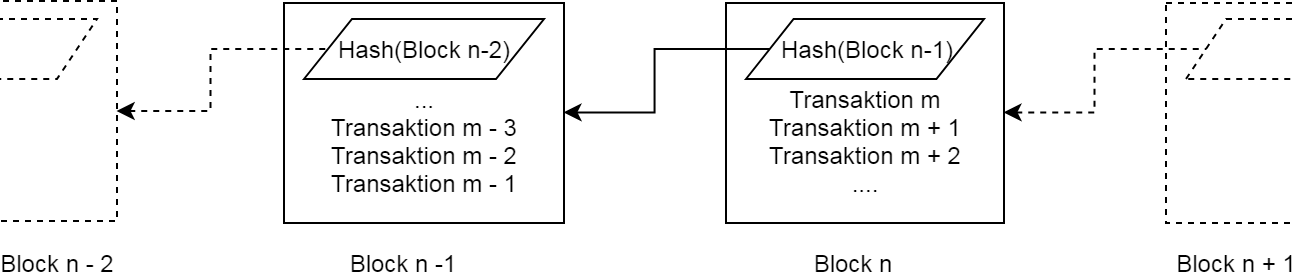
\includegraphics[width=\textwidth]{graphics/bc_highlvl.png}
    	\caption[Abstrakte Darstellung einer Blockchain]{Abstrakte Darstellung einer Blockchain. Jeder neu hinzugefügte Block (hier immer rechts angehängt) enthält eine Referenz auf den Vorigen mittels dessen Hashwert.}
    	\label{fig:bc_highlvl}
    \end{figure}
    \noindent Erstmals 2008 von Satoshi Nakamoto, ursprünglich als Peer-to-Peer Electronic Cash System ,,Bitcoin``
    \!\footnote{Heute werden Bitcoin, Ether, Ripple und andere als digitale Zahlungsmittel als sogennante Kryptowährung bezeichnet} 
    erfunden, erregte die Technologie aufgrund ihrer Eigenschaften wie ihres dezentralen, anonymen Konzepts schnell Aufmerksamkeit.\todo[color=orange]{Referenz} 
    Bitcoin ist die erste populäre digitale Währung, die ohne zentrale Autorität wie beispielsweise einer \gls{ttp} das in \fref{sec:sota_doublespend} vorgestellte Double-Spending Problem lösen sollte\cite{Nakamoto2008}. 
    Übertragen auf Bitcoin bedeutet es, dass ein Empfänger einer Transaktion sichergehen können muss, dass der vorige Besitzer den Bitcoin oder den Bruchteil dessen vorher nicht schon einmal erfolgreich an einen anderen Empfänger gesendet hat.
    Dies wird mittels kryptographischem Beweis, welcher in \fref{sec:sota_blockchain_consensus} genauer betrachtet wird, anstatt des laut \citeauthor{Nakamoto2008} vorstellten mangelhaften Modells dker \gls{ttp}, welche stets einen Single Point of Failure
    \!\footnote{Ein Single Point of Failure stellt beipsielsweise eine Bank im Zahlungsverkehr dar.
    Fällt die Bank beispsielsweise aus irgendeinem Grund aus oder wird kompromittiert, haben deren Kunden keine Möglichkeit mehr (sicher) Überweisungen auszuführen und zu empfangen.}
    darstellt, gelöst. 
    Das Konzept ermöglicht es somit zwei Entitäten, auch, wenn sie sich gegenseitig nicht vertrauen, ohne vermittelnde Person oder Organisation eine sichere (im Sinne der Integrität) direkte Transaktionen miteinander durchzuführen, welche auch im Nachhinein nicht mehr verändert werden können.\cite{Christidis2016}
    
    \subsubsection{Einführung in das Konzept}
    \label{sec:sota_blockchain_introduction}
    Grundlegend ist die Blockchain eine verteilte Datenstruktur, die zwischen den Mitgliedern eines Netzwerkes repliziert und geteilt wird\cite{Christidis2016}.
    Die Blockchain beinhaltet das maßgebliche ,,Hauptbuch`` (im Englischen ,,Ledger`` genannt) mit allen vergangenen Transaktionen, ein Log, dessen Einträge mit Zeitstempeln jeweils zu unterschiedlichen Blöcken zusammengefasst werden. 
    Alle vergangenen Transaktionen in der Reihenfolge ihres Auftretens sind für alle Teilnehmer einsehbar\cite{Nakamoto2008}.
    \medskip\\
    Nutzer nehmen an dem Netzwerk über Knoten teil, wobei ein Knoten auch für mehrere Nutzer einen Zugang bieten kann(s. \fref{fig:bc_network}). 
    Knoten des Netzwerkes speichern stets eine eigene Kopie der Blockchain.
    Jeder Nutzer interagiert mit dem Netzwerk mittels eines Paares von öffentlichem und privatem Schlüssel, wobei der Öffentliche oder dessen Hashwert zur Adressierung und der Private zur Signierung von Transaktionen des Nutzers verwendet wird.\cite{Christidis2016}
    \begin{figure}[H]
    	\centering
    	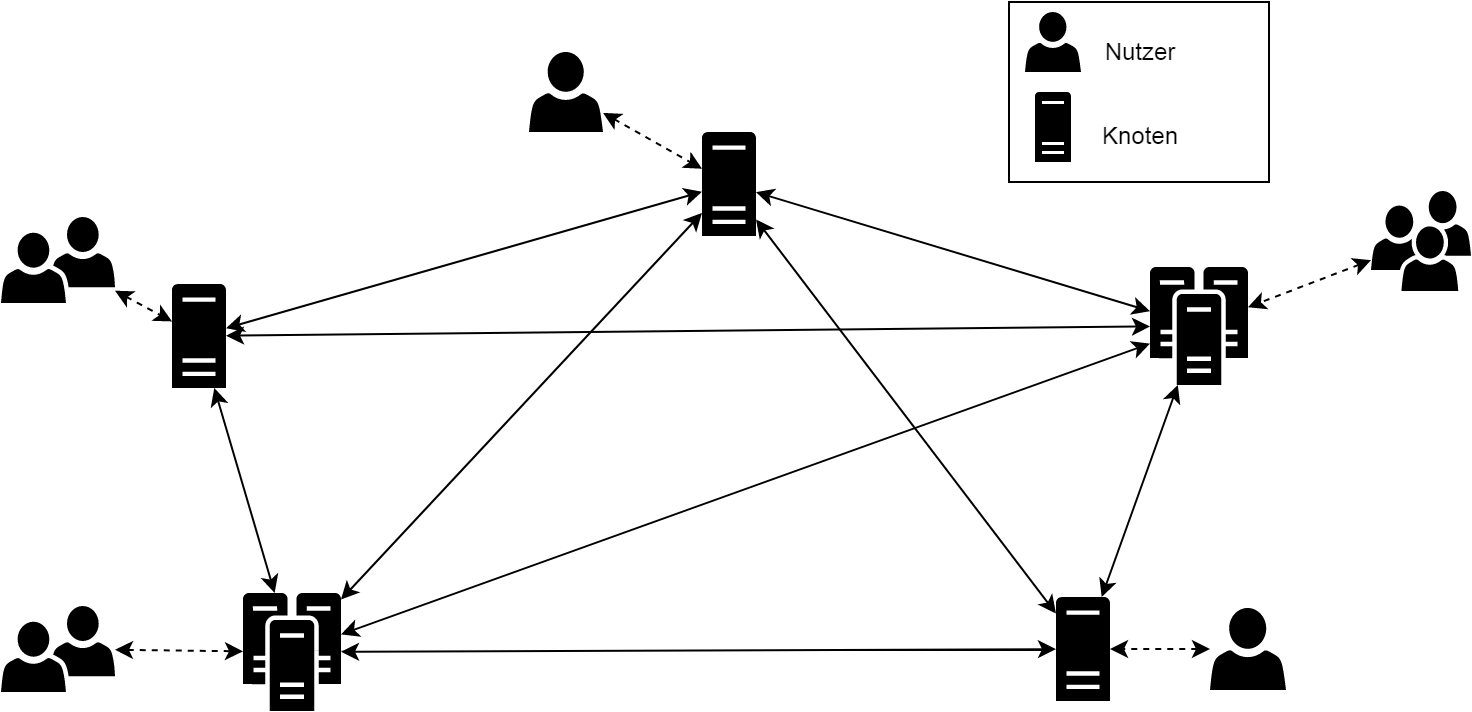
\includegraphics[width=\textwidth]{graphics/BCNetwork.png}
    	\caption[Blockchain-Netzwerk]{Blockchain-Netzwerk}
    	\label{fig:bc_network}
    \end{figure}
    
    Zunächst wurde mit digitalen Coins gehandelt, welche einer in Form einer Kette digitaler Signaturen modelliert wurden\cite{Nakamoto2008}.
    In anderen Anwendungsbereichen außerhalb des Bereiches der Kryptowährungen wird von generalisierten Assets gesprochen.
    Der aktuelle Zustand (,,World View`` genannt) ergibt sich also durch das Zurückverfolgen der einzelnen Transaktionen in der Blockchain. 
    Es wird also kein aktueller Stand, welcher Teilnehmer des Netzwerks was und wie viel besitzt, gespeichert.\cite{Christidis2016}
    
    \subsubsection{Transaktionen}
    \label{sec:sota_blockchain_trx}
    In einer Blockchain werden Aktivitäten von Nutzern in Form von Transaktionen repräsentiert. 
    
    Tätigt ein Nutzer eine Transaktion \lstinline{X}, so signiert er diese mit seinem privaten Schlüssel, der Knoten, über welchen der Nutzer mit dem Netzwerk interagiert, validiert diese, sammelt diese und verteilt die valide Transaktion an die nächsten Nachbarn
    \!\footnote{Nächste Nachbarn sind jene Knoten, die einen Sprung im \gls{p2p}-Netzwerk voneinander entfernt sind.}.
    Die Nachbarn überprüfen die Transaktion ebenfalls auf deren Validität und verbreiten diese wiederrum an ihre nächsten Nachbarn. 
    Schlussendlich kennen eine Vielzahl von Knoten im Netzwerk die Transaktion \lstinline{X}. 
    Das hierfür verwendete Protokoll wird als ,,Gossip-Protokoll`` bezeichnet.\cite{Christidis2016}
    
    Im sogenannten ,,Mining``-Prozess, der wiederholt wird, werden valide Transaktionen, die innerhalb eines im Voraus abgestimmten Zeitintervalls gesammelt wurden, zeitlich geordnet, zu einem mit Zeitstempel versehenem ,,Candidate``-Block zusammengefügt und wieder im Netzwerk verbreitet. 
    Andere Knoten im Netzwerk stellen sicher, dass der neue Block valide Transaktionen enthält und den richtigen Hash des vorigen Blocks in der Kette enthält. 
    Bei erfolgreicher Validierung hängen die Knoten den Block jeweils an ihre Kopie der Kette an, übernehmen die darin enhaltenen Transaktionen und aktualisieren somit den aktuellen Zustand. 
    Sollte innerhalb des Mining-Prozesses eine Validierung fehlschlagen, wird der ganze Block verworfen.\cite{Christidis2016}
    
    Der Knoten, der diesen Prozess ausführt wird Miner genannt und von der Auswahl des Knotens und Konsensmechanismus abhängig und unter Umständen in der gleichen Situation unterschiedlich.\cite{Christidis2016}
    
    \begin{figure}[H]
    	\centering
    	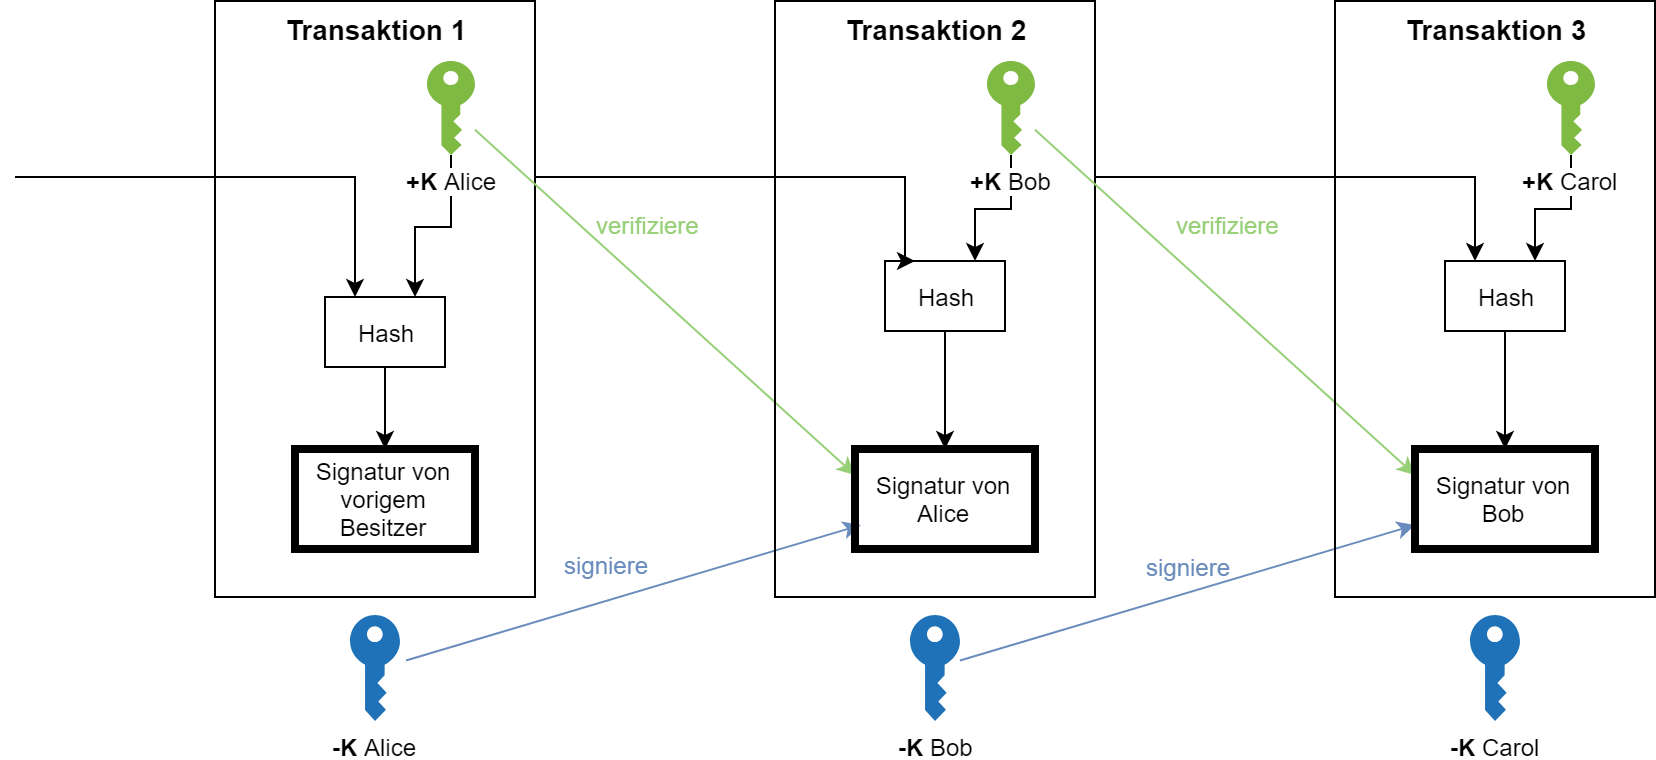
\includegraphics[width=\textwidth]{graphics/transaction.png}
    	\caption[Kette digitaler Signaturen]{Kette digitaler Signaturen\cite{Nakamoto2008}. \lstinline{+K} stellt dabei den öffentlichen und \lstinline{-K} den privaten Schlüssel dar.}
    	\label{fig:txio}
    \end{figure}
    
    Wie in \fref{fig:txio} dargestellt, werden Assets von einem Versender zu einem Empfänger transferiert, in dem der Sender einen Hash der vorigen Transaktion und den öffentlichen Schlüssel des Empfängers mit seinem eigenen privaten Schlüssel digital signiert und diese Hash dann am Ende des Assets anfügt.
    Der Empfänger, sowie alle Teilnehmer des Netzwerkes können den Besitz des Assets über die Kette der digitalen Signaturen zurückverfolgen.
    Transaktionen können zudem mehrere Ein- und Ausgaben haben.\cite{Nakamoto2008}
    
    Getätigte Transaktionen sollen nicht mehr rückgängig gemacht werden können.
    Erreicht wird dies, indem die Rückrechnung des Beweises rechnerisch zu aufwändig sein soll\cite{Nakamoto2008}.
    Somit wird der Verkäufer vor Täuschung geschützt und Treuhandmechanismen können einfach implementiert werden\cite{Nakamoto2008}.  
    \medskip\\
    Wie in \fref{fig:txio} dargestellt, werden Assets von einem Versender zu einem Empfänger transferiert, in dem der Sender einen Hash der vorigen Transaktion und den öffentlichen Schlüssel des Empfängers mit seinem eigenen privaten Schlüssel digital signiert und diese Hash dann am Ende des Assets anfügt.
    Transaktionen können zudem mehrere Ein- und Ausgaben haben\cite{Nakamoto2008}.
    
    Der Empfänger, sowie alle Teilnehmer des Netzwerkes können den Besitz des Assets über die Kette der digitalen Signaturen zurückverfolgen\cite{Nakamoto2008}.
	
	\subsubsection{Typen}
    \label{sec:sota_blockchain_types}
        Mit einer Blockchain können auch je nach Anwendungsszenario, außer Kryptowährungen, andere (als Token  repräsentierte) Waren oder Assets wie Güter im Supply Chain Management\cite{Underwood2016}, Identitäten zur Zugangskontrolle\cite{Kshetri2017} oder Proof of Ownership digitaler Rechte\cite{Wuest2017} gespeichert und gehandelt werden. 
        Unterschiedliche Anwendungen haben auch verschiedene Anforderungen an die Blockchain selbst. 
        Bei Anwendungen wie Supply Chain Management rückt beispielsweise der Aspekt ohne \gls{ttp} auszukommen eher in den Hintergrund. 
        Wichtig ist dort eher die Unveränderbareit und Nachverfolgbarkeit von Transaktionen in der Blockchain, die dabei helfen den Weg von Gütern von Start zum Ziel nachvollzeihbar zu machen. 
        Zur Zeit haben sich unterschiedliche Typen einer Blockchain herauskristallisiert, welche je nach Autor teilweise verschieden bezeichnet werden.
        Nach \cite{Wuest2017,Christidis2016,Buterin2015,Vukolic2017} wird in unterschiedliche Typen unterschieden:
        \begin{enumerate}[noitemsep]
            \item \textbf{public/permissionless}, Beispiele: Bitcoin, Ethereum\\
                Jeder kann zu einem beliebigen Zeitpunkt dem Netzwerk beitreten oder es verlassen und kann sowohl lesen, als auch schreiben und an dem Prozess der Konsensfindung teilnehmen. 
                Es existiert keine zentrale Autorität, welche die Mitgliedschaft im Netzwerk verwaltet und beispielsweise Teilnehmer, die aufgrund ihrer Handlungen ausgeschlossen werden sollen, verbannen könnte. 
            \item \textbf{public/permissioned} (auch Konsortium genannt), Beispiele: Microsoft Azure Coco\\
                Eine Gruppe von Organisationen oder eine Menge ausgeswählter Knoten reguliert und verwaltet eine Liste der Teilnehmer des Netzwerkes und deren Berechtigungen (lesen/schreiben), verifiziert Transaktionen und vollzieht den Miningprozess. 
                Somit können die einzelnen Transaktionen schneller überprüft, an die Blockchain angehängt und somit ausgeführt werden als bei einer öffentlichen Blockchain.
            \item \textbf{private/permissioned}, Beispiele: Hyperledger Fabric\\
                Ähnlich den public/permissioned Blockchains werden auch private von mindestens einer zentralen Autorität verwaltet, welche sich innerhalb einer einzelnen Organisation befindet.
        \end{enumerate}
	
    \subsubsection{Konsens und Sicherheit}
    \label{sec:sota_blockchain_consensus}
        Um Transaktionen selbst zu validieren, deren Reihenfolge im nächsten Block zu bestimmen und Mining-Blöcke auszuwählen zu können wird von allen Teilnehmern des Netzwerkes ein gemeinsamer Konsens vorausgesetzt. 
        Ist dies nicht der Fall können, wie in \fref{fig:bc_forks} dargestellt, unterschiedliche Ketten (,,Forks`` genannt) innerhalb der jeweiligen Kopien der Blockchain auf den einzelnen Knoten entsehen. 
        
        \begin{figure}[H]
        	\centering
        	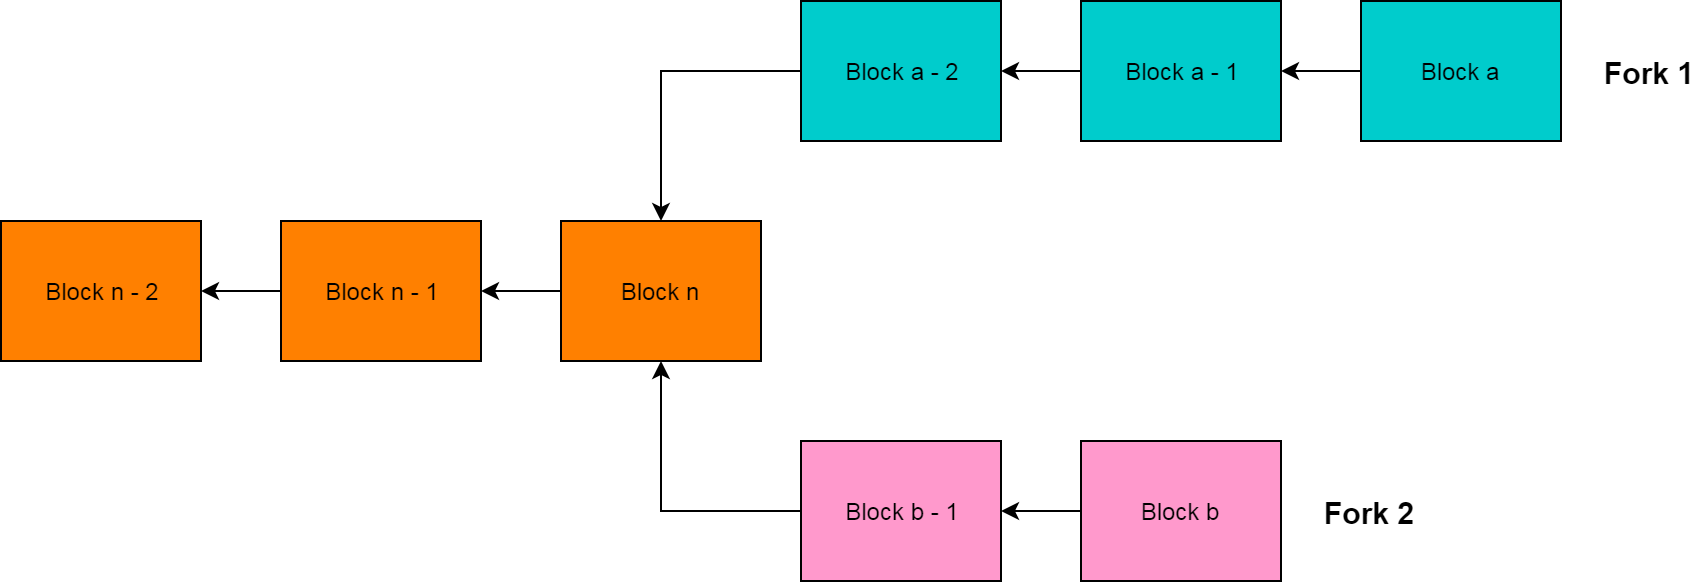
\includegraphics[width=\textwidth]{graphics/BCForks.png}
        	\caption[Blockchain mit Forks]{Blockchain mit zwei Forks}
        	\label{fig:bc_forks}
        \end{figure}
        \noindent Ideal wäre es, wenn alle validierenden Knoten des Netzwerkes abstimmen und die Mehrheit über die Reihenflolge der Transaktionen für den nächsten Block entscheidet.\cite{Christidis2016} 
        Aufgrund der Gefahr eines ,,Sybil-Angriffs``\cite{Trifa2014}
        \!\footnote{Bei einem ,,Sybil-Angriff`` erlangt ein Angreifer mehr Einfluss auf die Abstimmung, indem er entweder zusätzliche Nutzeridentitäten für sich selbst erstellt oder mehrere Knoten kontrolliert.
        } ist dies jedoch unzumutbar.
        Um diese Gefahr zu umgehen werden unterschiedliche Methoden angewendet, von denen einige Ausgewählte kurz erläutert werden:\cite{Christidis2016}
        \smallskip\\
        Bei Bitcoin wird ein sogenannnter \gls{pow} verwendet. 
        Das Mining wird rechnerisch ,,teuer`` gemacht, indem vorausgesetzt wird, dass ein minender Knoten eine richtige Zufallszahl (genannt ,,Nonce``) mit variablem Schwierigkeitsgrad und mit bestimmten Eigenschaften berechnet und mit einer bestimmten Anzahl Bitcoins belohnt wird. 
        Da bei der Berechnung kryptographische Hashfunktionen verwerndet werden, kann das Ergebnis durch die anderen Knoten einfach verifiziert werden. 
        Diese Zahl kann jeder Knoten im Netzwerk berechnenn, sodass die explizite Auswahl des Miners entfällt. 
        Der Candidate-Block jenes Knotens, der den Nonce findet, wird an die Blockchain angehängt. 
        Sollten Forks entstehen, wird der Fork verwendet, in der der meiste Rechenaufwand steckt. 
        Oft sind dies entweder der längste Fork oder der Fork, mit dem höchsten Schwierigkeitsgrad.\cite{Christidis2016,Nakamoto2008}
        \smallskip\\
        Alternativ kann ein \gls{pos} verwendet werden, welcher bedeutend weniger Rechenaufwand erfordert. 
        Dabei senden sich Besitzer selbst eine bestimmte Anzahl an Coins und addieren einen vordefinieren Prozentsatz als Belohnung. 
        Analog zum \gls{pow} wird ein Hashwert, entweder größer oder kleiner als ein gesuchter Wert ist berechnet, wobei die Schwierigkeit der Berechnung (umgekehrt proportional zum Alter der Coins) individuell festgelegt wird. 
        Der Hashwert wird aus statischen Daten, ausgenommen des Zeitstempels, berechnet, sodass bei jeder Änderung des Zeitstempels eine Chance zum Finden des Hashwertes besteht und die individuelle Rechenleistung der Knoten nur eine minimale Rolle spielt. 
        Wird ein Wert gefunden, so wird die Belohnung an den minenden Knoten ausgeschüttet und das Alter der Coins zurückgesetzt.\cite{Tschorsch2016}
        \medskip\\
        \gls{pow} und \gls{pos} werden vornehmlich in public (permissionless) Netzwerken eingesetzt.
        Für private Blockchains sind sie jedoch eher ungeeignet, da in solchen Netzwerken die Teilnehmer häufig per Whitelist bekannt sind. 
        In solchen Fällen werden Algorithmen wie das Practical \gls{bft} angewendet. Es löst das Problem der byantinischen Generäle
        \!\footnote{TODO
        } in asynchronen Umgebungen. 
        Es schließt ein Protokoll mit drei Phasen ein, sowie der Idee eines Primärknotens, welcher als Block Miner agiert. 
        Der Primärknoten kann über eine ,,View-Change``-Abstimmung geändert werden, falls dieser ausfällt oder sich willkürlich verhält (byzantinischer Fehler).
        Jedoch wird bei diesem Algorithmus davon ausgegangen, dass sich weniger als ein Dittel der Knoten fehlerhaft verhalten.
        \cite{Christidis2016}
    
    \subsubsection{Smart Contracts}
    \label{sec:sota_blockchain_sc}
        Smart Contracts sind Skripte, die innerhalb einer Blockchain gespeichert werden (ähnlich der Stored Procedures eines Relationalen Datenbankmanagementsystems) und agieren autonom. 
        Sie haben eine eigene Adresse und werden angesteuert, indem sie als Empfänger einer Transaktion adressiert werden.
        Die Ausführung passiert unabhängig automatisch und mit vorgegebenem Verhalten auf jedem Knoten des Netzwerks. \cite{Christidis2016}
        \smallskip\\
        Ein Beispiel für einen Smart Contract ist die Überprüfung von Transaktionen. 
        Dabei wird beispielsweise kontrolliert, ob der Sender mindestens die Anzahl an digitalen Token besitzt, die bei der Transaktion an den Empfänger übertragen werden sollen.
    
    \iffalse
    \subsubsection{Sicherheit}
    \label{sec:sota_blockchain_security}
        \begin{itemize}
            \item Users interact with the blockchain via a pair of private/public keys [13]. They use their private key to sign their own transactions, and they are addressable on the network via their public key.2 The use of asymmetric cryptography brings authentication, integrity, and nonrepudiation into the network\cite{Christidis2016}
            \item sonst noch was?
        \end{itemize}
    
    \subsubsection{Identity Management}
    \label{sec:sota_blockchain_identitymgmnt}
        ??
    \fi

    %\subsection{Internet of Things}
\label{sec:sota_iot}
\subsubsection{Sicherheit}
\label{sec:sota_iot_security}
\subsubsection{Protokolle (BLE, Z-WAVE)}
    \cite{Gomez2012}
    In \cite{Rose2016}
    \begin{itemize}
        \item nur kleine Datenmengen können ausgetauscht werden (20Bytes)\cite{Rose2016}
        \item geriner Energieverbrauch
        \item funktioniert wie Bluetooth Classic auf 2,4Ghz
        \item kurze Reichweite (<100m)
        \item verschiedene Hosts mit jeweils verschiedenen Profilen, geht vom Controller aus
    \end{itemize}
    
    \paragraph{Profile}\cite{Rose2016}
        \begin{itemize}
            \item General Attribute Profile (Client schickt Anfrage an GATT Server, Server speichert Attribute)
        \end{itemize}

\label{sec:sota_iot_protocols}
\subsubsection{Smart Home}
\label{sec:sota_iot_smart_home}
    \subsection{Smart Locks}
\label{sec:sota_smart_locks}
	Da sich Architektur und Funktionsmechanismen in manchen Punkten je nach Hersteller unterscheiden, gelten die im Folgenden dargelegten technischen Erklärungen, soweit nicht explizit erwähnt, für das Smart Lock von der Firma August. 
    \medskip\\
    \noindent Smart Locks sind ,,elektromechanische Türschlösser``, die sich dadurch auszeichnen, dass sie für einen Nutzer mit einer Smartphone-App steuerbar sind und mittels eines kabellosen Standards wie Bluetooth (siehe \fref{sec:sota_iot_protocols}) für kurze Distanzen kommunizieren.
	Als ,,Smart Lock`` werden keine Schlösser bezeichnet, bei denen ein physisches Schloss
	\footnote{beispielweise ein Stiftschloss, welches mit einem herkömmlichen Schlüssel geöffnet werden kann} 
	mit einem Ziffernblock ersetzt wurde oder sich nicht mit anderen Geräten innerhalb des \gls{iot} in irgendeiner Weise verbinden.\cite{Ho2016}
	
	\begin{figure}[H]
		\centering
		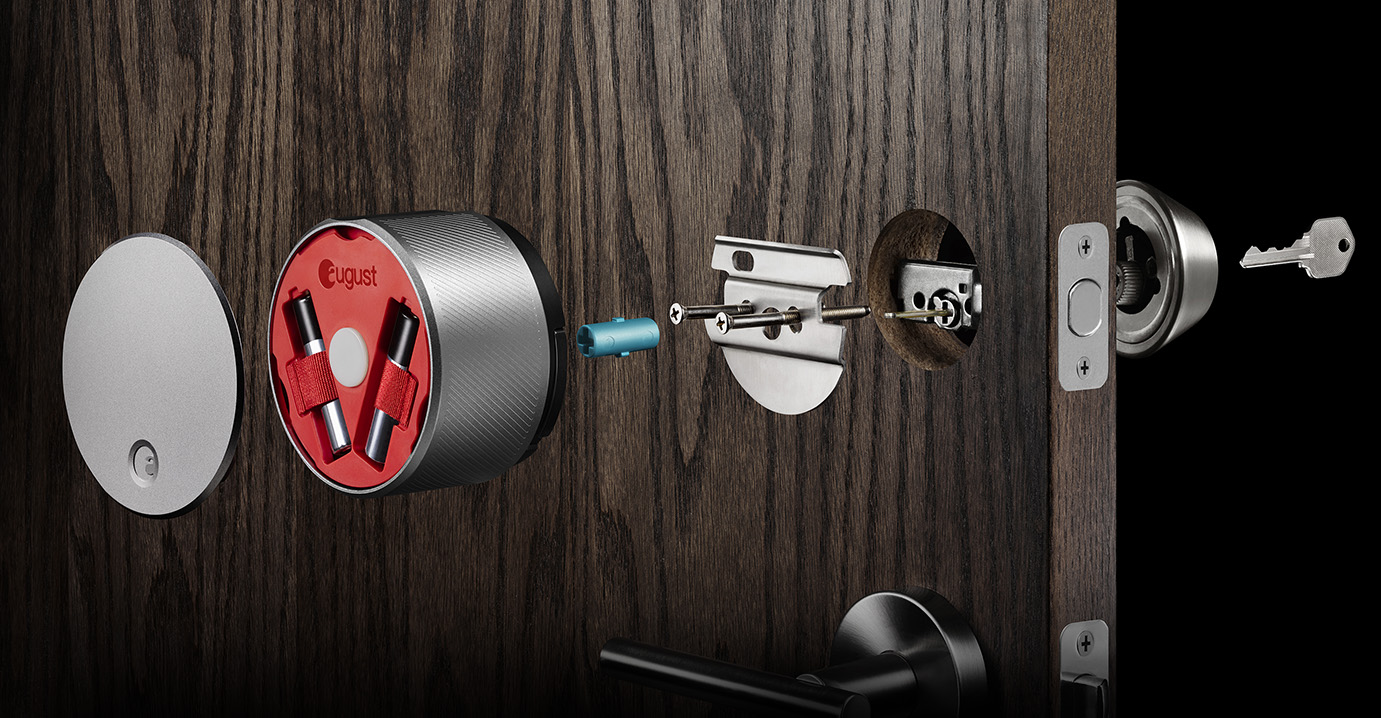
\includegraphics[width=0.9\textwidth]{graphics/august_2.jpg}
		\caption{Bestandteile eines August Smart Lock Pro\cite{August}}
		\label{fig:august1}
	\end{figure}
	
	\subsubsection{Typische Architekturen und Gemeinsamkeiten}
	\label{sec:sota_smart_locks_arch}
	    In den den doch sehr unterschiedlichen Produkten, die momentan auf dem freien Markt verfügbar sind oder bisher verfügbar waren, lassen sich trotz alledem einige Gemeinsamkeiten erkennen\cite{Ye2017,Fuller2017}. 
    	\noindent Generell besteht ein Smart Lock-System aus folgenden Bestandteilen (vgl. \fref{fig:sl_arch}):
    	\begin{enumerate}[noitemsep]
    		\item einem elektrischen Schloss oder einer elektronischen Erweiterung eines vorhandenen Schlosses
    		\item mindestens einem Nutzer, welcher durch sein Endgerät, meist ein Smartphone, identifiziert wird
    		\item einem oder mehreren herstellereigenen Servern
    		\item einem Webinterface
    		\item optional einem Zubehörgerät, welches dem Schloss als Gateway dient und es somit dem Schloss erlaubt mit dem Internet bzw. mit den Servern des Herstellers zu kommunizieren
    	\end{enumerate}
    
    	\begin{figure}[H]
			\centering
			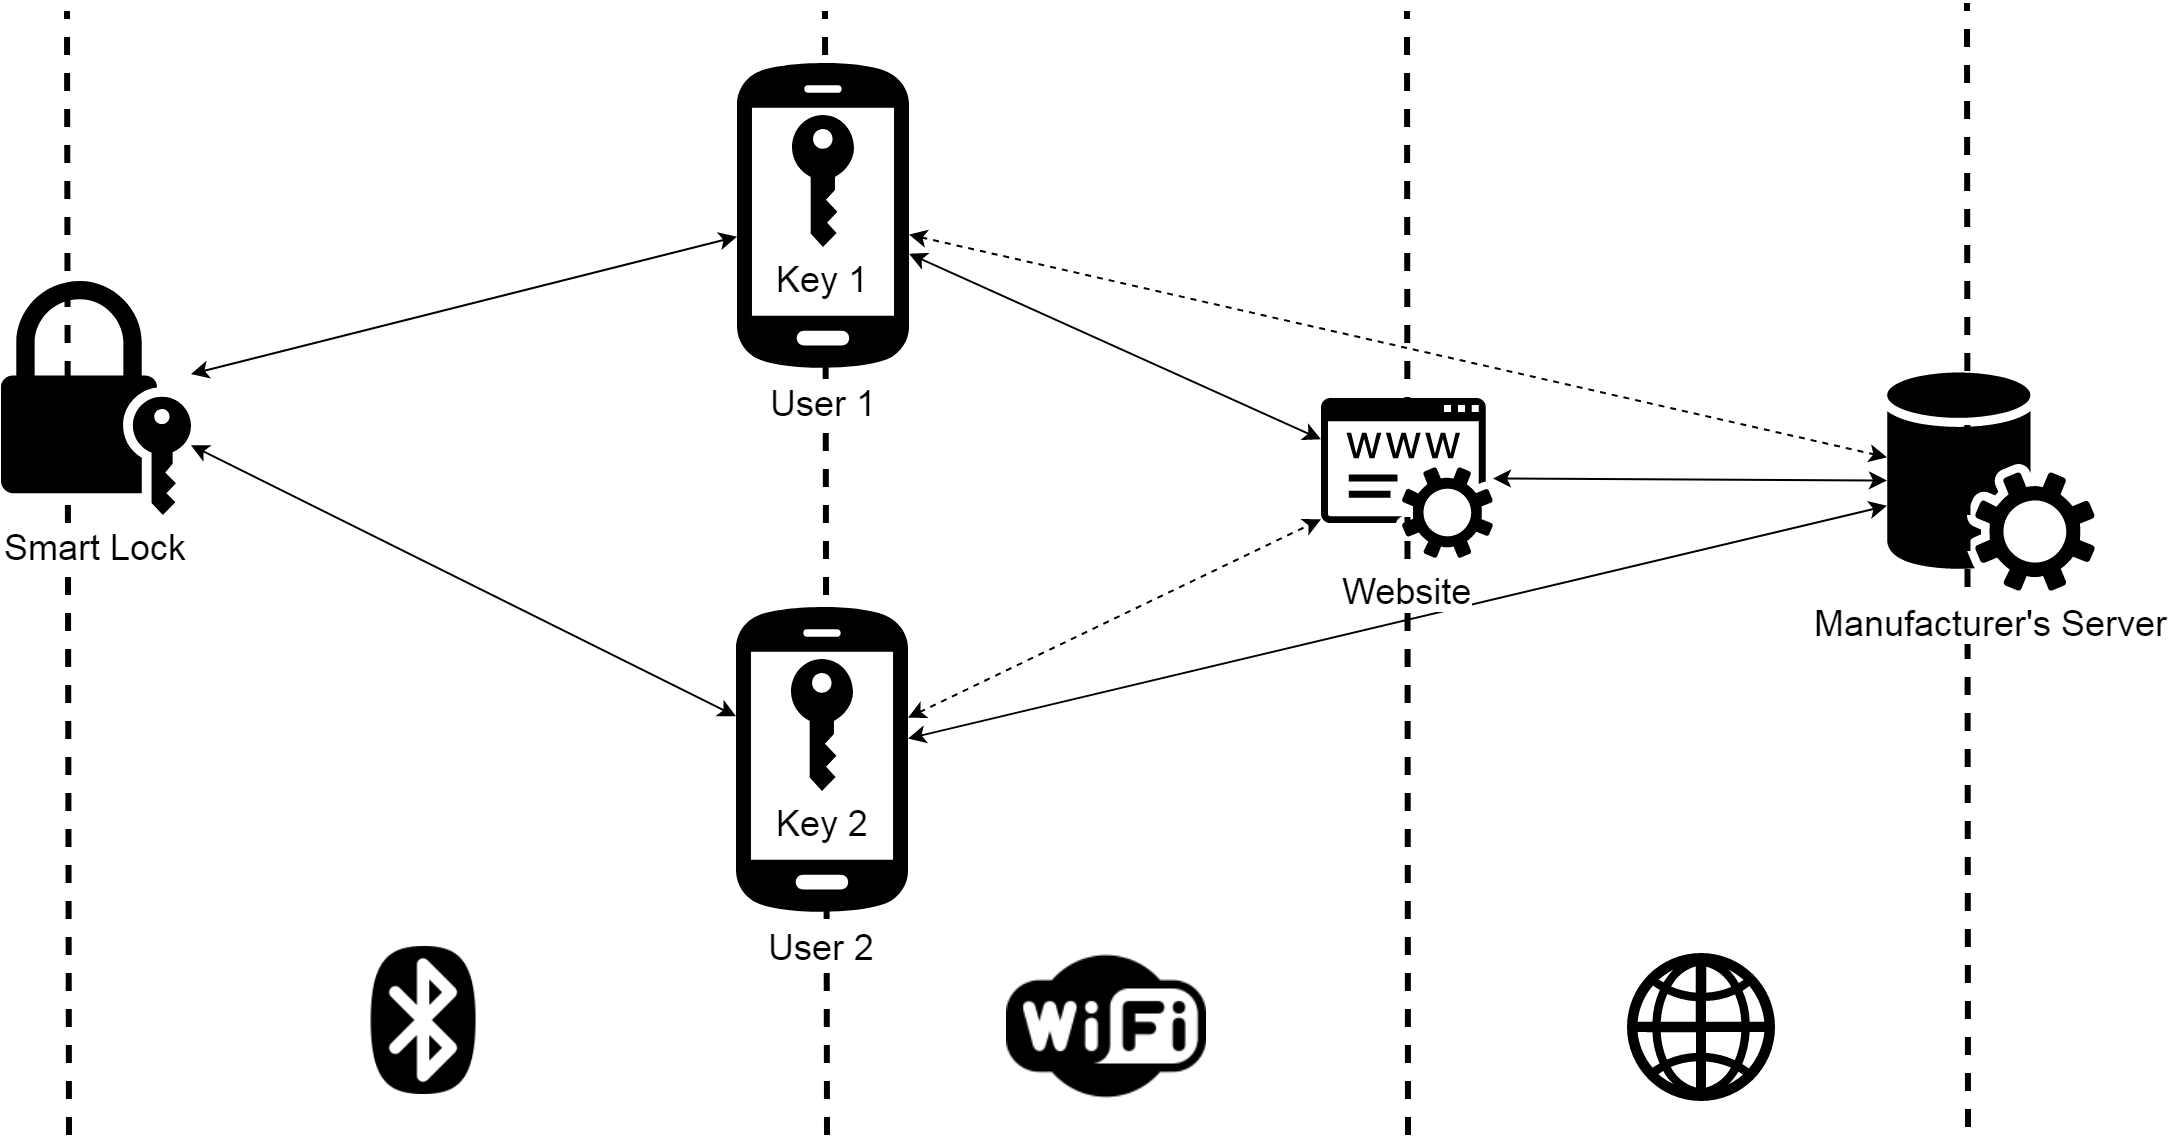
\includegraphics[width=\textwidth]{graphics/sl_arch.png}
			\caption{Beispiel eines Smart Lock-Systems}
			\label{fig:sl_arch}
		\end{figure}
    	
	    \noindent Das Schloss selbst ist an der Außen- und/oder Innenseite einer Tür angebracht (vgl. \fref{fig:august1}) und erweitert ein vorhandenes Schloss elektronisch oder ist selbst in Form eines Vorhängeschlosses\cite{Ho2016}. 
		Zum System gehört in den meisten Fällen eine mobile Applikation für ein Smartphone zum Öffnen und Schließen des Schlosses, sowie zur Administration\cite{Fuller2017}. 
        Eher seltener beinhaltet das Produkt auch eine Weboberfläche, welche ebenfalls für administrative Aufgaben genutzt werden kann\cite{Ho2016}. 
		Es existiert ein herstellereigener (Remote-)Server, auf dem sich eine authoritative Liste aller Nutzer, sowie deren Rechte befindet. 
        Diese bildet die Grundlage zur Realisierung der Zugriffskontrolle.\cite{Fuller2017} 
        Das Öffnen und Schließen erfolgt primär elektronisch mittels eines Buttons per App.
        Alternativ lässt sich das Schloss entweder mit einem sogenannten ,,Keyfob`` 
        \footnote{ein Schlüsselanhänger, auf dem sich ein digitaler Schlüssel befindet} 
        oder einem physischen Schüssel öffnen\cite{Ho2016}. 
        Einige Modelle bieten auch eine Funktion, die die Tür automatisch öffnet sobald sich der Nutzer innerhalb eines selbst festgelegten Geofencing-Radius befindet. 
        (Bei Geofencing wird mittels \gls{gps} ein Ort festgelegt, um den ein virtueller Zaun gelegt wird. 
        Verlässt oder betritt der Nutzer den festgelegten Radius um den Ort, wird ein Trigger ausgelöst, dem beliebige Aktionen folgen können.) 
        \smallskip\\
        \noindent Sobald folgende Bedingungen gegeben sind, kann sich das Schloss automatisch öffnen: 
        \begin{itemize}[noitemsep]
        	\item automatisches Öffnen wurde vom Nutzer aktiviert
        	\item der Nutzer hat einen Ort für das Geofencing festgelegt
        	\item der Nutzer befindet sich in \gls{ble}-Reichweite, um über sein Smartphone mit dem Schloss kommunizieren zu können
        	\item der Nutzer ist berechtigt das Schloss zu öffnen
        \end{itemize}
    	Verlässt der Nutzer den Radius des Geofencings wieder, wird das Schloss automatisch verriegelt. 
    	\smallskip\\
		Ein optionales Zubehörgerät, welches in \fref{fig:sl_arch} nicht dargestellt wird, fungiert als Relay
		\footnote{leitet Nachrichten von mehreren Entitäten in einem Netzwerk (unverändert) weiter}
		, welches sich per \gls{ble} mit dem Schloss verbindet und über das W-LAN Heimnetzwerk des Nutzers mit dem Internet verbindet.
		
    \subsubsection{Typische Funktionen}
    \label{sec:sota_smart_locks_func}
		Um das Schloss zu kontrollieren installiert der Nutzer initial eine herstellerspezifische App auf seinem Smartphone und erstellt ein Nutzerkonto auf dem Server des Herstellers. 
		Danach pairt der Nutzer via \gls{ble} sein Gerät mit dem Schloss.\cite{Ho2016} 
		Die Identifikation der verschiedenen Nutzer für administrative Zwecke erfolgt entweder mittels E-Mailadresse oder Telefonnummer. 
		Aus technischer Sicht werden Nutzer anhand eines einzigartiger Schlüssel identifiziert, die der Besitzer des Schlosses nicht kennt.\cite{Fuller2017}\todo[color=orange]{nachlesen} 
		Die Smart Locks enthalten eine eingebaute Funktion, um Zugriffe zu protokollieren. 
		Dazu gehören Aktionen wie \cite{Fuller2017}:
		\begin{itemize}[noitemsep]
			\item von welchem Nutzer eine Funktion genutzt wurde, 
			\item der Zeitpunkt, an dem das Schloss elektronisch geöffnet oder geschlossen wurde,
			\item der Zeitpunkt, an dem das Schloss manuell geöffnet oder geschlossen wurde
			\item wann, wem und von wem Zugriff gewährt oder entzogen wurde
		\end{itemize}
	
	\subsubsection{Kommunikation}
	\label{sec:sota_smart_locks_comm}
	    \begin{figure}[H]
    		\centering
    		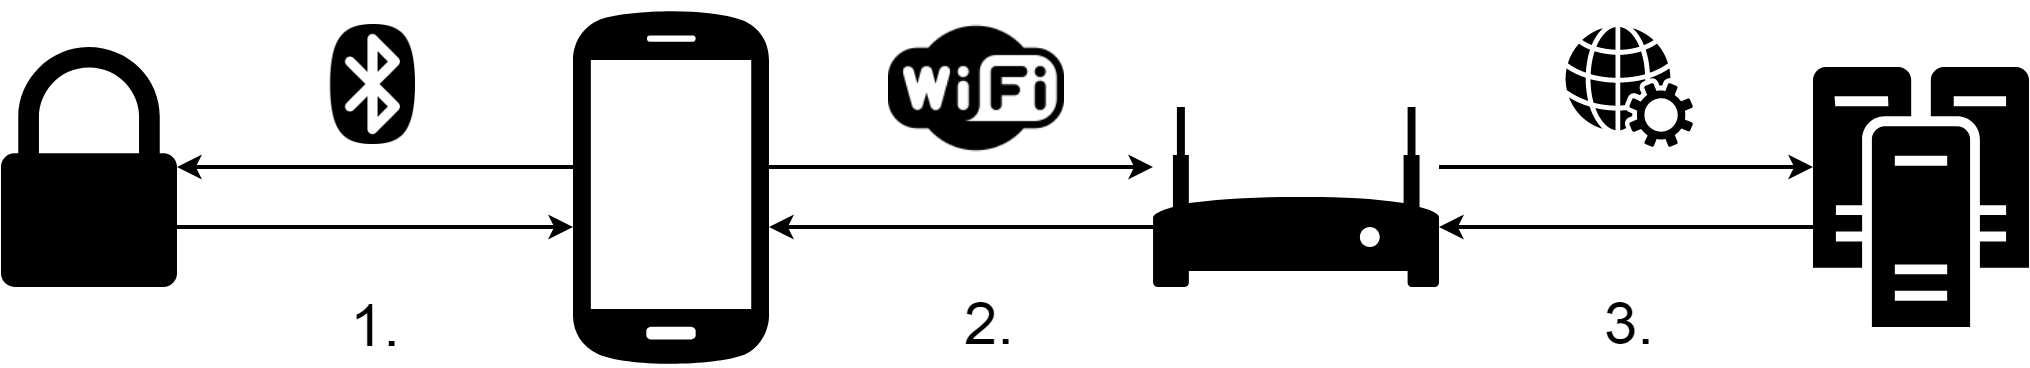
\includegraphics[width=0.9\textwidth]{graphics/gateway_arch.png}
    		\caption{Typische Architektur, welche das Smartphone des Nutzers als Gateway/Proxy nutzt\cite{Ho2016}.}
    		\label{fig:gateway_arch}
    	\end{figure}
	    Nach \cite{Ho2016}:
        In \fref{fig:gateway_arch} erkennbar ist, dass das Smart Lock selbst hat keine direkte Verbindung zum Internet oder den Servern des Herstellers hat. 
        Das Endgerät des Nutzers übernimmt die Funktion eines Gateways für die Verbindung zum Internet und Proxys zur Übertragung von Informationen zwischen dem Smart Lock und den Servern des Herstellers. 
        Dies setzt voraus, dass sich das Endgerät in Kommunikationsreichweite von \gls{ble} befindet. 
        \smallskip\\
        Übertragen über \gls{ble} werden Informationen wie beispielsweise
        \begin{itemize}[noitemsep]
            \item Die in \fref{sec:sota_smart_locks_comm} beschriebenen Logdateien werden asynchron mit den Servern des Herstellers aktualisiert, sobald sich das Gerät des Nutzers in Reichweite des \gls{ble} befindet.
            \item Nachrichten mit Informationen über gewährten und entzogenen Nutzerrechten
            \item Athentifizierung des Smartphones des Nutzers 
        \end{itemize}
        
        \noindent Einige andere Modelle wie Lockitron\cite{lockitron} nutzen eine direkte Internetverbindung des Smart Locks zur Kommunikation mit den Servern des Herstellers. 
        Dabei baut das Schloss mittels eingebautem Wifi-Modem eine Verbindung mit dem Netzwerk des Nutzers auf und kommuniziert so mit den Servern. 
        Die übertragenen Informationen wie Rechtevergaben und Gerätezustand werden hier direkt über das Internet und nicht über lokale Kommunikation (wie \gls{ble}) übertragen. 

    \subsubsection{Sichereit}
    \label{sec:sota_smart_locks_sec}
        Häufig kommt für die Zugangskontrolle ein rollenbasiertes Konzept zum Einsatz. 
        Jeder Rolle werden bestimmte Rechte (vgl. \fref{tab:rbac}) zugeordnet.\cite{Ye2017,Ho2016,Fuller2017} 
		\begin{table}[H]
		    {\footnotesize
		    \centering
            \begin{tabular}{|m{0.114\textwidth}|m{0.114\textwidth}|m{0.114\textwidth}|m{0.114\textwidth}|m{0.114\textwidth}|m{0.114\textwidth}|m{0.114\textwidth}|}
            \hline
            \textbf{Rolle/Recht} & \textbf{Auto-Öffnen (de-)aktivieren} & \textbf{Lock/Unlock} & \textbf{Logdateien einsehen} & \textbf{Nutzer hinzufügen/löschen} & \textbf{Rollen\-verwal\-tung} & \textbf{Schloss kali\-brieren/zurück\-setzen} \\ \hline
            \textbf{Owner}      & \checkmark                   & \checkmark          & \checkmark           & \checkmark                         & \checkmark                    & \checkmark                           \\ \hline
            \textbf{Resident}   & \checkmark                   & \checkmark          & ~                    & ~                                  & ~                             & ~                                    \\ \hline
            \textbf{Guest}      & \checkmark                   & \checkmark          & ~                    & ~                                  & ~                             & ~                                    \\ \hline
            \end{tabular}
            }
            \caption{Beispiel einer rollenbasierten Zugriffskontrolle}
            \label{tab:rbac}
        \end{table}
		\normalsize
		\noindent In \fref{tab:rbac} nicht angegeben, aber dennoch für alle Rollen gültig: Jeder kann seinen eigenen Account löschen. 
		\begin{description}
		    \item [Owner] Die Rolle des Owners wird jenem Gerät vergeben, das sich nach Installation bzw. nach Zurücksetzen des Smart Locks als erstes mittels \gls{ble} verbindet. 
   		        Auf diesem Wege wird die Owner-Rolle nur einmal vergeben. 
   		        Bei Wechsel des Besitzers muss das Smart Lock zurückgesetzt werden. 
   		        Ein Owner kann allerdings auch die Rolle des Owner an andere Nutzer weitergeben, sowie diese wieder entziehen. 
   		        Um die Rechte eines Owners bei einem verlorenen oder gestohlenen zu entziehen, wird entweder eine ,,Lost Phone``-Funktion angeboten oder ein anderer Nutzer mit der Rolle des Owners entzieht dem nicht mehr vorhandenen Gerät die Rolle. 
   		        Der Owner kann das Schloss auch ohne Internetverbindung öffnen/schließen. 
   	        \item [Resident] Ein Bewohner kann das Schloss öffnen oder schließen. 
   	            Sollte die automatische Öffnen/Schließen-Funktion aktiviert werden, wird auch bei einem Bewohner das Schloss automatisch geöffnet und geschlossen. 
   	            Bewohner und Gäste müssen sich vor der Kommunikation mit dem Schloss gegenüber der dem Server des Herstellers autorisieren lassen.
   	        \item [Guest] Der Gast unterscheidet sich von einem Bewohner lediglich darin, dass er nur innerhalb eines begrenzten Zeitraums Zugang hat. 
                Der Zeitraum des Zugangs wird durch einen Owner festgelegt.
		\end{description}
        
		\paragraph{Secret Keys}\hspace{0pt}\smallskip\\
		Jede Bluetooth-Verbindungssession bekommmt einen eigenen einzigartigen \gls{sk}, welcher für Owner und Guest/Resident unterschiedlich entsteht.
		Dieser wird verwendet, um Nachrichten zwischen dem Schloss und dem Smartphone des Nutzers mit dem Verschlüsselungsalgorithmus \gls{aes} zu ver- und entschlüsseln. 
		Voraussetzung für das Protokoll, welches den Session Key erstellt ist, dass bereits im Voraus das Schloss und entweder die Webserver des Herstellers oder das Smartphone des Nutzers einen Secret Key teilen. 
		Dieser Secret Key ist beipsielsweise das Passwort, das der Nutzer während seiner Anmeldung in der App verwendet. 
		In dem Smart Lock von August können insgesamt 256 Schlüssel (von 0 bis 255 nummeriert) gespeichert werden, wobei Nummer 0 besondere Privilegien hat und als ,,Firmware Key`` angesehen wird.\cite{Fuller2017} 
		Im Fall von August ist der Key hardcoded und somit anfällig, sollte er in falsche Hände geraten\cite{Rose2016}. 
        Die restlichen 255 Keys sind ,,offline Keys``, die zur Initialisierung einer Bluetooth-Session verwendet werden, sollte der Nutzer nicht mit dem Internet verbunden sein.\cite{Fuller2017}
        
		\begin{figure}[H]
    		\centering
    		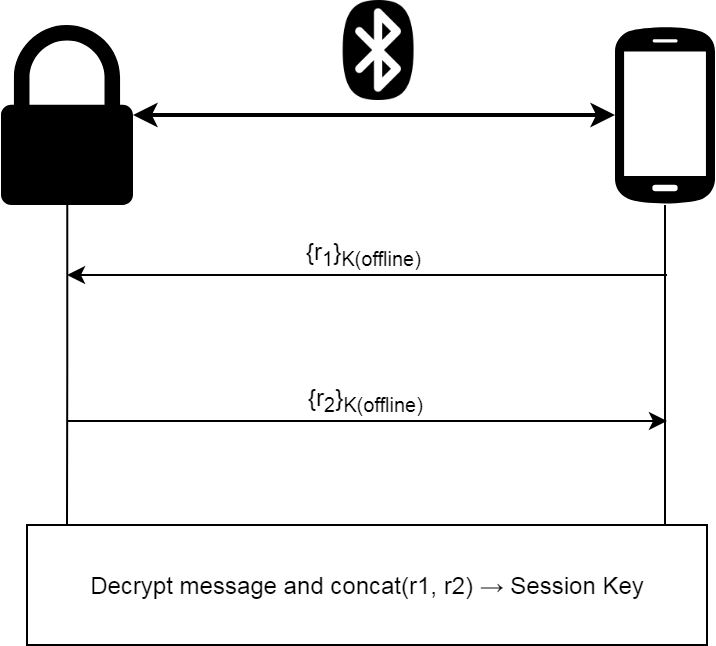
\includegraphics[width=0.6\textwidth]{graphics/owner_key.png}
    		\caption{Ablauf der Generierung eines \gls{sk} mittels offline Key\cite{Fuller2017}}
    		\label{fig:owner_key}
    	\end{figure}
		
		\noindent\fref{fig:owner_key}\todo[color=yellow]{bessere Überleitung}:
        \begin{enumerate}[noitemsep]
            \item das Smartphone sendet zufällige 64 Bit an das Schloss, welche mit dem offline Keys des Smartphones verschlüsselt werden, an das Schloss
            \item das Schloss sendet 64 zufällige Bits, die mit dem offline Key des Smartphones verschlüsselt sind, an das Smartphone zurück
            \item das Schloss und das Smartphone entschlüsseln die jeweils erhaltene Nachricht und konkatinieren beide Nachrichten zu einer neuen 128-Bit langen Folge, die im weiteren Verlauf als \gls{aes}-Key zur Verschlüsselung der Session genutzt wird
        \end{enumerate}
        
        \noindent Gäste, welche keinen ,,offline Key`` zugewiesen bekommen, kommunizieren mit dem Webserver (vgl. \fref{fig:online_key}):\todo[color=orange]{nachlesen}
        
        \begin{figure}[H]
    		\centering
    		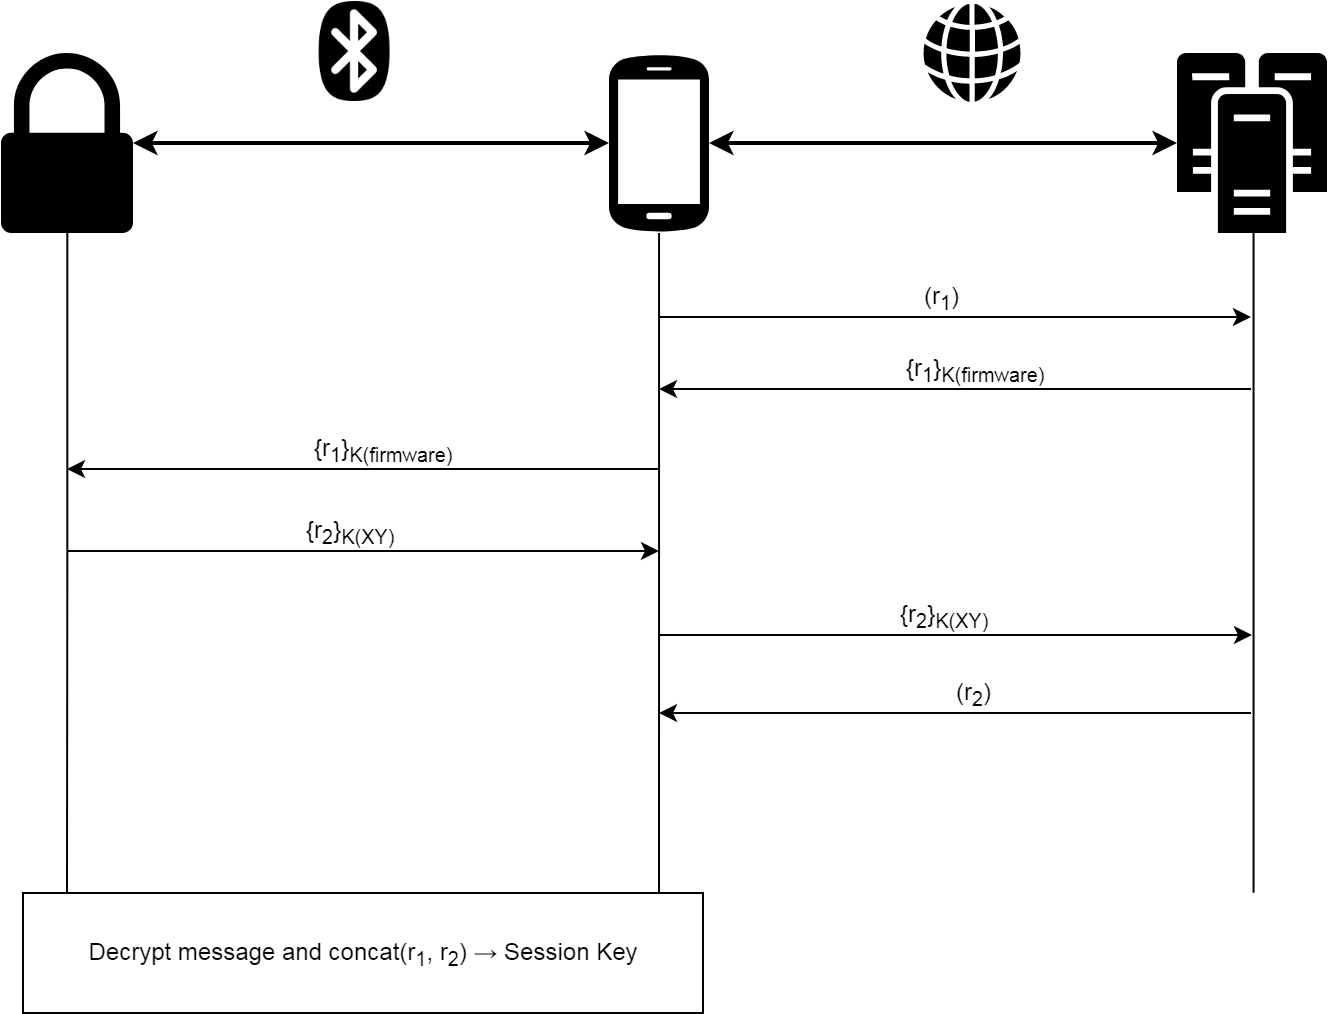
\includegraphics[width=0.9\textwidth]{graphics/online_key.png}
    		\caption{Ablauf der Generierung eines \gls{sk} ohne offline Key\cite{Fuller2017}}
    		\label{fig:online_key}
    	\end{figure}
        
        \begin{enumerate}[noitemsep]
            \item das Smartphone des Gasts sendet 64 zufällige Bits als Klartext an den Server
            \item der Server verschlüsselt diese 64 Bits mit dem Firmware Key und sendet die verschlüsselten Bits als Nachricht an den Gast zurück
            \item der Gast leitet den Ciphertext, welcher von dem Server empfangen wurde, an das Schloss weiter
            \item das Schloss sendet 64 Bits mit XY\todo[color=orange]{nachlesen} verschlüsselt an den Gast, welcher diesen Ciphertext an den Server weiterleitet
            \item Der Server entschlüsselt die Nachricht und sendet sie als Klartext per SSL an den Gast
            \item das Schloss und der Gast konkatenieren beide 64-Bit langen Folgen zu einem 128-Bit Schlüssel, welcher als Session Key verwendet wird
        \end{enumerate}

    \subsection{Vulnerability Assessment im Internet of Things}
\label{sec:sota_sa}
    Logisch gesehen kann das \gls{iot} als Sammlung von Smart Devices gehen werden, die kollaborativ auf ein gemeinsames Ziel hinarbeiten. 
    Technologisch gehen nutzen diese Geräte dafür unterschiedliche Kommunikationswege und -protokolle, basierend auf verschiedenen Architekturen und Mechanismen. 
    Dies führt dazu, dass ein hohes Level an Heterogenität herrscht. 
    Die Geräte haben zudem meist nur geringe Rechenleistung, sind aber dennoch untereinander stark vernetzt, wodurch sich die für einen Angreifer möglichen Angriffsvektoren vervielfacht und es erschwert traditionelle Sicherheitesmechanismen anzuwenden.\cite{Sicari2015}
    
    Um mögliche Schwachstellen in diesen komplexen Ökosystemen zu finden und zu vermeiden wurden vom \gls{owasp} mehrere Ressourcen veröffentlicht.
    Darunter befinden sich ein Dokument mit den Top 10 gefundenen Sicherheitslücken in \gls{iot}-Geräten\cite{Miessler2015}, sowie ein Testing Guide\cite{Miessler}, um ein Gerät systematisch zu untersuchen.
    
    
    Die gefundenen Schwachstellen werden als solche bezeichnet, sobald sie eines der klassischen Ziele\cite{Perrin2008} in der Informationssicherheit bedrohen. 
    Zu den Zielen gehören:
    \begin{itemize}[noitemsep]
        \item Vertraulichkeit: Zugriff und Preisgabe von Informationen ist nur auf autorisierte Entitäten limitiert.
        \item Integrität: Die Information ist vertrauenswürdig und integer, wurde als während einer möglichen Übertragung nicht verändert.
        \item Verfügbarkeit: Hiermit ist die Verfügbarkeit der Informatin gemeint, die beispielsweise von auf einem Webserver liegt.
    \end{itemize}
    
    \noindent In \cite{Sicari2015} werden die Ziele für das \gls{iot} erweitert. 
    Zusätzlich zu den o.g. Sicherheitszielen werden Folgende definiert:
    \begin{itemize}[noitemsep]
        \item Authentifizierung: Eine Entität muss verifizieren, dass sie auch die ist, als welche sie sich indentifiziert.
        \item Zugriffskontrolle: Verschiedene Entitäten haben verschiedene Autorisierungen, um verschiedene Informationen zu lesen oder schreiben.
        \item Non-Repudiation: Jegliche Änderungen an einer Information müssen auf die ändernde Entität zurückverfolgbar sein.
    \end{itemize}
	
	\noindent Um existierende Schwachstellen zu bewerten, kann ein Standard, wie das \gls{cvss} verwendet werden.
	
\subsubsection{Common Vulnerability Scoring System (CVSS)}
\label{sec:sota_sa_cvss}
    \todo[color=cyan]{System kurz erklären}
    The Common Vulnerability Scoring System (CVSS) provides a way to capture the principal characteristics of a vulnerability, and produce a numerical score reflecting its severity, as well as a textual representation of that score. The numerical score can then be translated into a qualitative representation (such as low, medium, high, and critical) to help organizations properly assess and prioritize their vulnerability management processes.
    Vorteile: standardized vulnerability scores, open framework, enables prioritized risk\cite{CVSSspec}
    
    
    \noindent Der Base Score besteht aus zwei Subscores, Exploitability Score und Impact Score, welche wie folgt in Listing \ref{eq:cvss_basescore} verrechnet werden:
    \begin{lstlisting}[caption={Berechnung des BaseScore \cite{CVSSspec}},label=eq:cvss_basescore,captionpos=b,mathescape=true]
if (ImpactSubScore <= 0)
    BaseScore = 0
else
if(Scope == Unchanged)
    BaseScore = RoundUp(Minimum [(Impact + Exploitability), 10])
if(Scope == Changed)
    BaseScore = RoundUp(
      Minimum [1.08 $\mathsf{\times}$ (Impact + Exploitability), 10])
    \end{lstlisting}
    
    \noindent Ziel des Base Scores ist es wesentliche Charakteristiken, die in verschiedenen Umgebungenen und Zeitpunkten konstant sind, einer Schwachstelle zu repräsentieren. 
    Der Score liegt zwischen dem Wert 0.0 und 10.0, wobei 0 das kleinste Risiko repräsentiert und 10 das Größte\cite{CVSSspec}. 
    Die \fref{tab:cvss_severity} zeigt die Zuordnung der verschiedenen Scores zu Risikograden. 
    \begin{table}[H]
        \centering
        \begin{tabular}{|m{0.2\textwidth}|m{0.2\textwidth}|}
        \hline
        \textbf{Rating}   & \textbf{\gls{cvss} Score}   \\ \hline
        None              & 0.0                         \\ \hline
        Low               & 0.1 - 3.9                   \\ \hline
        Medium            & 4.0 - 6.9                   \\ \hline
        High              & 7.0 - 8.9                   \\ \hline
        Critical          & 9.0 - 10.0                  \\ \hline
        \end{tabular}
        \caption[Skala des Ausmaßes einer ausgenutzten Schwachstelle]{Skala des Ausmaßes einer ausgenutzten Schwachstelle\cite{CVSSspec}}
        \label{tab:cvss_severity}
    \end{table}
    \noindent Der Exploitability Score wird aus den Exploitablility Metrics berechnet(vgl. Listing \ref{eq:cvss_explscore}) und modelliert die Charakteristiken der anfälligen Komponente. 
    \smallskip\\
    \begin{lstlisting}[caption={Berechnung des Exploitability Score \cite{CVSSspec}},label=eq:cvss_explscore,captionpos=b,mathescape=true]
Exploitability = 8.22 $\mathsf{\times}$ AttackVector $\mathsf{\times}$ AttackComplexity 
  $\mathsf{\times}$ PrivilegeRequired $\mathsf{\times}$ UserInteraction
    \end{lstlisting}
    \noindent Folgende Variablen werden dabei verrechnet:
    \begin{description}[itemsep=0.7em,align=left,labelindent=0pt,leftmargin=0pt]
        \item [Attack Vector:] Beschreibt den Kontext, in der Ausnutzung der Schwachstelle möglich ist.
            Der Wert, der in den Exploitability Score einfließt ist größert, je entfernter (im technischen Sinne) ein Angreifer sein kann, um einen Angriff zu starten.
            \begin{description}[noitemsep,align=left,labelindent=0.7cm,leftmargin=0.7cm]
                \item [Network:] Schwachstelle ist über Netzerkzugriff ausnutzbar, auch, wenn der Zugriff ein oder mehrere Hops via Layer 3
                \footnote{nach dem OSI-Modell}
                entfernt ist. 
                \item [Adjacent:] Schwachstelle ist über Netzerkzugriff ausnutzbar, aber der Angriff ist auf das selbse physische oder logische Netzwerk eingeschränkt und kann nicht über eine Layer 3 Grenze (bspw. einem Router) ausgeführt werden.
                \item [Local:] Ein lokaler Zugriff ist nötig, um die Schwachstelle ausnutzen zu können und die Komponente ist nicht an den Netzwerkstack gebunden.
                Der Angriff funktioniert über lesende/schreibende/ausführende Zugriffe und kann voraussetzen, dass der Angreifer entweder in das System eingeloggt ist und/oder eine Nutzerinteraktion tätigt, bei der eine bösartige Datei ausgefürt wird.
                \item [Physical:] Der Angreifer muss in der Lage sein die anfällige Komponente über eine bestimmte Zeit physisch zu bedienen oder zu manipulieren.
            \end{description}
        \item [Attack Complexity:] Beschreibt die Bedingungen außerhalb der Kontrolle des Angreifers, die herrschen müssen, um die Schwachstelle auszunutzen (bspw. bestimmte Systemkonfiguration).
            \begin{description}[noitemsep,align=left,labelindent=0.7cm,leftmargin=0.7cm]
                \item [Low:] Spezielle Zugriffsbedingungen oder ähnliches existieren nicht.
                Ein Angreifer kann wiederkehrenden Erfolg gegen die Komponente erzielen.
                \item [High:] Ein erfolgreicher Angriff hängt von Zuständen außerhalb des Einflusses des Angreifers ab und kann voraussetzen, dass der Angreifer im Voraus einiges an Aufwand investieren muss, um diese Zuständer herzustellen.
            \end{description}
        \item [Privileges Required:] Beschreibt das Level an Privilegien, die ein Angreifer besitzen muss, um eine Schwachstelle ausnutzen können.
            \begin{description}[noitemsep,align=left,labelindent=0.7cm,leftmargin=0.7cm]
                \item [None:] Der Angreifer ist vor dem Angriff nicht autorisiert und benötigt daher keinen Zugriff auf Einstellungen oder Dateien, um den Angriff ausführen zu können.
                \item [Low:] Der Angreifer ist mit grundlegenden Nutzerrechten autorisisiert.
                \item [High:] Der Angreifer ist mit erweiterten oder administrativen Rechten autorisiert und kann komponentenweite Einstellungen und Dateien ändern.
            \end{description}
        \item [User Interaction:] Beschreibt die Voraussetzung, ob ein Angreifer einen erfolgreichen Angriff ohne weitere Beteiligung von anderen Nutzern ausführen kann oder ob ein Nutzer in irgendeiner Weise mitwirken muss.
            \begin{description}[noitemsep,align=left,labelindent=0.7cm,leftmargin=0.7cm]
                \item [None:] Ein Angriff kann ohne Interaktion eines anderen Nutzers erfolgreich sein.
                \item [Required:] Erfolgreiches Ausnutzen einer Schwachstelle ist nur möglich, wenn ein anderer Nutzer eine oder mehrere bestimmte Aktionen ausführt.
            \end{description}
    \end{description}
    
    \noindent Der Impact Score wird aus den Impact Metrics berechnet (vgl. Listing \ref{eq:cvss_impscore} und beschreiben die Eigenschaften des betroffenen Komponenten. 
    Sollte ein erfolgreich ausgeführter Angriff auch andere Komponenten beeinflussen, so wird die Komponente mit dem worst-case, also der höchsten Einstufung gewertet.
    \smallskip\\
    \begin{lstlisting}[caption={Berechnung des Impact Score \cite{CVSSspec}},label=eq:cvss_impscore,captionpos=b,mathescape=true]
$\mathsf{ISC_{Base}}$ = 1 - [(1 - $\mathsf{Impact_{Conf}}$) $\mathsf{\times}$ (1 - $\mathsf{Impact_{Integ}}$) $\mathsf{\times}$ (1-$\mathsf{Impact_{Avail}}$)]
if (Scope == Unchanged)
    Impact = 6.42 $\mathsf{\times}$ $\mathsf{ISC_{Base}}$
if (Scope == Changed)
    Impact = 7.52 $\mathsf{\times}$ [$\mathsf{ISC_{Base}}$ - 0.029] - 3.25 $\mathsf{\times}$ [$\mathsf{ISC_{Base}}$ - 0.02]$\mathsf{^{15}}$
    \end{lstlisting}
    \begin{description}[itemsep=0.7em,align=left,labelindent=0pt,leftmargin=0pt]
        \item [Confidentiality:] Ausmaß auf die Vertraulichkeit der Informationsressourcen, die von einer Softwarekomponente verwaltet werden, welche durch das Ausnutzen einer Schwachstelle komprommittiert wurde.
            \begin{description}[noitemsep,align=left,labelindent=0.7cm,leftmargin=0.7cm]
                \item [None:] Kein Verlust der Vertraulichkeit.
                \item [Low:] Der Angreifer erlangt eingeschränkt Zugriff auf Informationen, hat aber keine Kontrolle darüber, welcher Informationen er erlangt.
                    Oder: Die Preisgabe der Informationen verursacht keinen direkten, schweren Verlust bei der betroffenen Konponente.
                \item [High:] Die Vertraulichkeit ist nicht mehr gegeben.
            \end{description}
        \item [Integrity:] Ausmaß auf die Integrität der Informationsressourcen, die von einer Softwarekomponente verwaltet werden, welche durch das Ausnutzen einer Schwachstelle komprommittiert wurde.
            \begin{description}[noitemsep,align=left,labelindent=0.7cm,leftmargin=0.7cm]
                \item [None:] Kein Verlust der Integrität.
                \item [Low:] Änderung von Daten durch einen Angreifer ist möglich, aber der Angreifer selbst hat keine Kontrolle über die Konsequenz seiner Modifikation oder das Maß der Modifikation ist eingeschränkt.
                \item [High:] Verlust jeglicher Integrität.
                    Der Angreifer kann alle Daten, die durch die Komponente geschützt oder kontrolliert werden modifizieren.
            \end{description}
        \item [Availability:] Ausmaß auf die Verfügbarkeit der Informationsressourcen, die von einer Softwarekomponente verwaltet werden, welche durch das Ausnutzen einer Schwachstelle komprommittiert wurde.
            Damit ist der Verlust der Verfügbarkeit der betroffenen Komponente (wie ein Webservice, eine Datenbank, etc.) selbst gemeint.
            \begin{description}[noitemsep,align=left,labelindent=0.7cm,leftmargin=0.7cm]
                \item [None:] Kein Verlust der Verfügbarkeit
                \item [Low:] Reduzierte Leistung oder Unterbrechungen in der Verfügbarkeit der Ressource.
                \item [High:] Kompletter Verlust der Verfügbarkeit, was dazu führt, dass ein Angreifer den Zugriff auf Ressourcen innerhalb der betroffenen Komponente verhindern kann.
            \end{description}
    \end{description}
    
    \begin{description}[itemsep=0.7em,align=left,labelindent=0pt,leftmargin=0pt]
        \item [Scope:] Beeinflusst ein erfolgreicher Angriff mindestens eine andere Komponente außer die Anfällige?
            \begin{description}[noitemsep,align=left,labelindent=0.7cm,leftmargin=0.7cm]
                \item [Unchanged:] Eine ausgenutzte Schwachstelle beeinflusst nur Ressourcen, die von der gleichen Authorität verwaltet werden - anfällige und die betroffene Komponenten sind also identisch.
                \item [Changed:] Eine ausgenutzte Schwachstelle kann Ressourcen außerhalb der Komponente beeinflussen - anfällige und die betroffene Komponenten sind also nicht identisch.
            \end{description}
    \end{description}
    
    \noindent Es existieren Erweiterungen des Base Scores, der Temporal Score und Environmental Score. 
    Diese beiden Werte werden in dieser Arbeit nicht verwendet. 
    Für die genauen Werte, die für die Berechnungen verwendet werden, wird auf \cite{CVSSspec} verwiesen.\todo[color=cyan]{Anhang?}
    
    \newpage
    \section{Analyse}
\label{sec:analysis}
	Um spezielle Anforderungen für den Prototypen festlegen zu können, werden zunächst bekannte Sicherheitslücken von bestehenden Produkten analysiert. 
	Als Schwachstellen und Sicherheitslücken werde jene aufgenommen, die zumindest in einem Produkt entdeckt und vor dem Zeitpunkt der Erstellung dieser Arbeit veröffentlicht wurden.
	Zunächst werden einige bekannte Schwachstellen und/oder Sicherheitslücken kurz vorgestellt.
	Um die Basis für eine Vergleichbarkeit zwischen vorhandenen Produkten und dem in dieser Arbeit entwickelten Prototypen zu gewährleisten, werden gefundene Schwachstellen und Sicherheitslücken kategorisiert und nach dem \gls{cvss}-Basis Score bewertet.
	Aus diesen Ergebnissen lassen sich einige spezielle Anforderungen an den Prototypen ableiten, die in \fref{sec:analysis_requirements} erwähnt werden.
	\todo[color=green]{KL}

    \subsection{Bekannte Schwachstellen und Angriffe}
\label{sec:analysis_vulns}
    Es werden nach Literaturrecherche hier einige Schwachstellen und Angreiffe vorgestellt. 
    Die Kategorisierung nach den \gls{owasp} Top Ten \gls{iot} Vulnerabilities\cite{Miessler2015}. 
    Sollte eine Schwachstelle in mehrere Kategorien passen, so wird sie in jene eingeordnet, in der der größte Schaden im Falle eines Angriffs entsteht.\todo[color=yellow]{besser formulieren}
    Für weitere Details zu den im Folgenden beschriebenen Schwachstellen wird auf die jeweiligen Quellen verwiesen.
    \todo[color=orange]{\cite{Tierney2018}\cite{Stykas2018}}

    \subsubsection*{I1: Insecure Web Interface}
       \begin{itemize}[leftmargin=0cm,label={}]
            \item \emph{Insecure API: User Enumeration}\cite{Fuller2017,Lariviere2015}\label{vuln:userenum}\\
                Produkt: August\\
                Voraussetzungen: \\
                Die in \fref{sec:sota_smart_locks} vorgestellte Kommunikation via Wifi zwischen dem Webserver: 
                Wenn sich ein Nutzer das erste Mal in der App anmeldet, wird eine zufällige ID generiert (installID), welche an den Webserver gesendet wird und für viele API-Aufrufe entweder als Teil des API-Keys oder zusätzlich zu diesem verwendet wird. 
                Die API Endpunkte authentifizieren den Nutzer nicht und erlauben es einem Angreifer einen Gästezugang anzulegen, wenn dieser die \gls{uuid} kennt.
                Diese kann wiederrum durch das Nutzen einer Funktion in der Smartphone-App, welche nach Smart Locks in Reichweite sucht, erlangt werden. 
       \end{itemize} 
       
    \subsubsection*{I2: Insecure Authentification/Authorization}
        \begin{itemize}[leftmargin=0cm,label={}]
            \item \emph{Insufficient Password Protection}\cite{Ye2017}\label{vuln:pwdprot}\\
    	        Produkt: QuickLock Smart Lock\\ 
                Voraussetzungen: keine\\
                Wird die ,,Passwort vergessen``-Funktion genutzt, so wird dem Nutzer sein verwedetes Passwort zugesendt. 
                Das übertragene Passwort wird allerdings nicht verschlüsselt.
            \item \emph{Insecure API: Privilege Escalation}\cite{Fuller2017,Lariviere2015}\label{vuln:privesc}\\
                Produkt: August\\
                Voraussetzungen: \\
                Die in \fref{sec:sota_smart_locks} vorgestellte Kommunikation via Wifi zwischen dem Webserver: 
                Ebenfalls möglich war eine Privilege Escalation, in dem ein String von 'user' auf 'superuser' geändert wurde.
            \item \emph{Insecure Password Policy}\cite{Rose2016,Ye2017,Jmaxxz2015a}\label{vuln:pwdpol}\\
                Produkt: Quicklock Smart Lock, August Smart Lock\\
                Voraussetzungen: keine\\
                Quicklock: 8-Ziffern PIN (100.000.000 Kombinationen)\\
                August: Verifikation über Rufnummer enthält einen Code mit 6 Ziffern (1.000.000 Kombinationen)\\
                Sollte kein Rate-Limiting im Server vorhanden sein, könnte der Angreifer mit beispielsweise 50 Versuchen pro Sekunde (bei 20ms Netzwerkverzögerung) ide 1.000.000 Kombinationen innerhalb von maximal 5-6 Stunden knacken.
            \item \emph{Phishing?}\cite{Ye2017}\label{vuln:phishing}\\
    	        Produkt: August Smart Lock\\ 
                Voraussetzungen: keine\\
                Der Angreifer bringt den Nutzer dazu eine bösartige App zu verwenden, welche der Legitimen sehr ähnlich sieht. 
                Da keine Authentifizierung zwischen Schloss und Nutzer durchgeführt wird, ist dies nur sehr schwer vom Nutzer zu erkennen.
            \item \emph{Replay}\cite{Tierney2018,Rose2016,Ho2016}\label{vuln:replay}\\
                Produkt: Tapplock Smart Lock, Ceomate Bluetooth, Elecycle Smart Padlack, Vians Bluetooth Smart Doorlock, Lagute Sciener Smart Doorlock\\
                Voraussetzungen: \\  
                Vom Nutzer übertragene Befehle zwischen Smartphone und Schloss werden eine Zeit lang aufgezeichnet und zu einem späteren Zeitpunkt wieder abgespielt. 
                Hat sich der Nutzer innerhalb dieser Zeitspanne beispielsweise gegenüber dem Schloss authentifiziert, so kann sich der Angreifer mit dem abgespielten Befehl als der Nutzer authentifizieren.\todo[color=yellow]{doof formuliert}
                Ein Angreifer folgt Alice (außerhalb des Bluetooth- und Geofencingradius, aber in Bluetooth-Reichweite zu Alices Gerät) und überträgt das Signal an einen anderen Angreifer, der vor Alices Haus mit einem bluetoothfähigen Gerät wartet und mittels des übertragenen Signals nun alle Bedingungen erfüllt und das Schloss entriegeln kann.
                Bei Systemen mit Geofencing muss zusätzlich Alices Standort gespooft werden.
            \item \emph{Device Spoofing}\cite{Rose2016}\label{vuln:spoofing}\\
                Produkt: Mesh Motion Bitlock Padlock\\
                \begin{enumerate}[noitemsep]
    	            \item Angreifer gibt sich als Schloss aus, um das Passwort des Nutzers zu stehlen
    	            \item möglich, da ein vorhersehbarer Nonce geschickt wird und die App beim Nutzer im Hintergrund läuft und Befehle ohne Nutzerinteraktion sendet.
    	        \end{enumerate}
	        \item \emph{Missing 2-Factor Authentication}\cite{Jmaxxz2015}\label{vuln:2factor}\\
                Produkt: August Smart Lock\\
                Voraussetzungen: \\  
                Proof of Posession: E-Mail, Handynummer\\
                Proof of Knowledge: Passwort
                \begin{enumerate}[noitemsep]
                    \item Nutzer benutzt die ,,Passwort vergessen`` Funktion auf einem Smartphone, auf dem der Nutzer bereits mindestens einmal angemeldet war.
                    \item Hersteller sendet Token an die E-Mailadresse des Nutzers.
                    \item Nutzer kann sein Passwort ändern.
                \end{enumerate}
                \begin{enumerate}[noitemsep]
                    \item Nutzer nutzt die ,,Passwort vergessen`` Funktion auf einem Smartphone, auf dem noch kein Nutzer angemeldet war.
                    \item Hersteller sendet Token an E-Mailadresse und Rufnummer des Nutzers.
                        Der Token, der der Rufnummer zugesandt wird muss vor dem Zurücksetzen des Passwortes eigegeben werden.
                    \item Um in dieser Situation zwei Faktoren zur Authentifizierung zu haben, müsste laut \cite{Jmaxxz2015} die Kontrolle über die Rufnummer oder die E-Mailadresse als Proof of Knowledge gelten.
                        Wird eines der beiden Faktoren als Proof of Knowledge defniniert erhält man einen Widerspruch und somit auch keine Authentifizierung über zwei Faktoren, sondern nur über einen Faktor.
                \end{enumerate}
        \end{itemize}
        
    \subsubsection*{I3: Insecure Network Services}
        \begin{itemize}[leftmargin=0cm,label={}]
            \item \emph{Denial of Service via Commands}\cite{Ye2017}\label{vuln:doscmd}\\
    	        Produkt: August Smart Lock \\ 
                Voraussetzungen: Angreifer hat Zugriff auf das Smartphone eines Nutzers und auf dem Smartphone selbst Root-Rechte\\
                Winn mehrere Nutzer gleichzeitig versuchen sich mit dem Schloss zu verbinden, wird die App suspendiert, sodass niemand gleichzig Öffnen/\-Schließen-Befehle senden kann. 
    		    Somit kann ein Angreifer kontinuierlich wechseln Öffnen/Schließen-Befehle senden und der legitime Nutzer kann die Smart Lock nicht kontrollieren. 
		    \item \emph{Denial of Service (via manufacturer's server)}\cite{Ye2017}\label{vuln:dosserver}\\
                Produkt: Lockitron\\
                Voraussetzungen: im WLAN Bereich des Nutzers
                direkte Verbindung des Schlosses mit den Servern des Herstellers \textrightarrow legitime Nutzer könnten ausgeschlossen werden, wenn dessen Server nicht erreichbar sind
            \item \emph{Denial of Service via Bluetooth}\cite{Ye2017}\label{vuln:dosble}\\
    	        Produkt: alle\\ 
                Voraussetzungen: keine\\
                Der Angreifer nutzt einen Bluetooth-Jammer, um die Kommunikation zwischen Smartphone und Schloss zu unterbinden. 
                Aufgrund der in \fref{fig:gateway_arch} vorgestellten Architektur sind somit keine Dienste mehr verfügbar. 
            \item \emph{Access Log Evasion}\cite{Ho2016}\label{vuln:accesslogevasion}\\
                Produkt: August, Danalock, Kevo, Okidokeys, Lockitron\\
                Voraussetzungen: \\
                ist möglich, da, wie in dem oben beschriebenen Szenario davon ausgegangen wird, dass alle Geräte alle Aktionen an den remote Server senden.
                Szenario mit Danalock: Alice, Bob und Mallory haben einen legitimen Zugang.
                Bob ist Owner und kann die Access Logs einsehen.
                Mallory blockiert alle Pakete, die von der App an den remote Server gesendet werden während er mit dem Schloss via ÖFFNEN/\-SCHLIEßEN- Befehl interagiert.
                Somit werden seine Aktionen nicht mitgeschrieben, da das Schloss selbst diese Aktionen von Schloss selbst nicht zwischengespeichert und über einen anderen Client an den remote Server gesendet werden.
                Da diese Informationen auch nachdem Alice mit dem Schloss interagiert nicht über ihr Gerät an den Server weitergeleitet werden, kann Bob als Owner nicht sehen, dass Mallory das Schloss geöffenet oder geschlossen hat.
        \end{itemize}
        
    \subsubsection*{I4: Lack of Transport Encryption/Integrity Verification}
        \begin{itemize}[leftmargin=0cm,label={}]
            \item \emph{Insecure Password Transmission}\cite{Rose2016}\label{vuln:pwdtrns}\\
                Produkt: Quicklock, iBluLock, Pantraco Phantomlock\\
                Voraussetzungen: \\ 
                Plain Text Password: z.B. einfach Opcode (Herstellserspezifisch), aktuelles Passwort, neues Passwort konkatiniert und gesendet. 
    	        Wird dies gesendet, dann wird der Owner mit einem neuen Passwort ausgesperrt und ein hard Reset ist nötig. 
    	        Jedoch ist diser Angriff nur möglich, wenn das Schloss in dem Moment, in dem die Nachricht gesendet wird, entriegelt ist.
            \item \emph{Insecure Bluetooth-Pairing - Session Key}\cite{Fuller2017}\label{vuln:blesk}\\
                Produkt: August\\
                Voraussetzungen: \\
                der Session Key wird als Klartext vom Server an den Gast geschickt, sodass ein Mithörer an diesen gelangen könnte.
    	        Er wird jedoch unverzüglich für die Kommunikation zwischen Schloss und Gast genutzt und direkt nach Nutzung wieder verworfen, sodass das Kennen des Session Keys für einen Angreifer laut \citeauthor{Fuller2017} eher unwahrscheinlich einen Nutzen hervorbringt.
	        \item \emph{Revocation Evasion}\cite{Fuller2017,Ho2016}\label{vuln:revocationevasion}\\
                Produkt: August, Danalock, Kevo, Okidokeys, Lockitron\\
                Voraussetzungen: \\
                Indem ein Angreifer, dessen Rechte entzogen werden soll jegliche Kommunikation zwischen Alice und dem remote Server des Herstellers verhindert.
                Dies kann beispielsweise am einfachsten mittels des Flugmodus erreicht werden.
                Gleichzeitig entgeht der Angreifer auch dem Access Logging.
                Szenario mit Danalock: Alice möchte Mallory, einem Nutzer mit temprärem Zugang die Rechte entziehen. 
                Dazu nutzt sie die App, welche diese Information an den Server des Herstellers sendet und ihr sofort bestätigt, dass sie Rechte von Mallory nun entzogen wurden. 
                Dieser sendet eine Benachrichtigung darüber an Mallorys Gerät. 
                Befindet sich Mallorys Gerät zu diesem Zeitpunkt im Flugmodus, erreicht diese Benachrichtigung ihr Ziel nicht und das Schloss selbst bleibt unwissend über dieses Ereignis. 
                Selbst, wenn ein legitimes Gerät mit dem Schloss interagiert, wird die Benachrichtung über Mallorys Entzug der Recht nicht vom Server über jenes übertragen.
                Somit behält Mallory Zugang für das Schloss. 
                Oder: in Angreifer mit einem in der Zukunft auf Zeit limitierten Gastzugang ändert die Zeiteinstellung auf seinem Gerät, um zu einem anderen Zeitpunkt Zugriff zu erhalten
            \item \emph{Decompiling APKs}\cite{Rose2016}\label{vuln:decompile}\\
                Produkt: Poly-Control Danalock Doorlock\\
                Voraussetzungen: \\  
                \begin{enumerate}[noitemsep]
    	            \item APKs vom Android-Gerät holen
    	            \item .dex zu .jar konvertieren
    	            \item .jar dekompilieren
    	            \item zeigt Verschlüsselungsmethode und hardcoded Secret (Kerckoff's Prinzip)
    	            \item XOR(passwort, secret) \textrightarrow es ist also einfach an das Passwort zu kommen \textrightarrow Entschlüsseln der Kommunikation ist möglich
    	        \end{enumerate}
        \end{itemize}
        
    \subsubsection*{I5: Privacy Concerns}
        \begin{itemize}[leftmargin=0cm,label={}]
            \item \emph{Extracted User Data}\cite{Lariviere2015,Ye2017}\label{vuln:userdata}\\
                Produkt: August Smart Lock\\ 
                Voraussetzungen: Angreifer hat Zugriff auf das Smartphone eines Nutzers\\
                Jegliche gesammelten persönlichen Informationen, die für die Anmeldung der App benötigt werden, werden auf dem Smartphone des Nutzers mit \gls{aes} verschlüsselt abgelegt. 
                Der verwendete Modus der \gls{aes}-Versclüsselung ist \gls{ecb}, wobei der verwendete Schlüssel hardcoded und als Klartext in der Smartphone-App abgelegt wird. 
    		    Ein Angreifer, der Zugriff auf das Smartphone von Alice hat, kann also u.a. UserId, Namen, Rufnummer und Profilbild von Alice auslesen.
        \end{itemize}
        
    \subsubsection*{I6: Insecure Cloud Interface}
        \begin{itemize}[leftmargin=0cm,label={}]
            \item 
        \end{itemize}
        
    \subsubsection*{I7: Insecure Mobile Interface}
        \begin{itemize}[leftmargin=0cm,label={}]
            \item \emph{Stolen User Settings}\cite{Ye2017}\label{vuln:usersettings}\\
                Produkt: August Smart Lock\\ 
                Voraussetzungen: Angreifer hat Zugriff auf das Smartphone eines Nutzers und auf dem Smartphone selbst Root-Rechte\\
                Mallory kopiert die Einstellungen der App, welche als eine bestimmte Datei auf dem Smartphone von Alice gespeichert werden.
    		    Mallory legt sich einen neuen Account an und nutzt dafür die kopierten Einstellungen. \textrightarrow Mandatory Access Control 
    		    Nun wird der Angreifer als legitimer Nutzer angesehen.
    		    Dies beinhaltet die Verwendung von jeglichen administrativen Funktionen wie das Ändern der Gästeliste. 
		    \item \emph{Insecure Bluetooth-Pairing}\cite{Tierney2018,Rose2016,Ye2017,Fuller2017}\label{vuln:blepairing}\\
                Produkt: August Smart Lock, Tapplock Smart Lock\\
                Voraussetzungen: keine\\
                August: Das Bluetooth-Pairing zwischen Schloss und Alices Smartphone wird über die Passkey-Methode vollzogen. 
                Der verwendete Handshake-Key ist statisch und ist in den Dateien, welche die Einstellungen der App enthalten, als Klartext auf Alices Smartphone zu finden. 
                Zudem wird keine Authentifizierung zwischen beiden Entitäten durchgeführt und in den Zugriffsprotokollen ist nicht erkennbar, dass ein Angreifer mit dem Schloss interagiert hat. 
                Kann exploited werden (mit Proof of concept auf Github)\\
                Tapplock: Der Key für das Bluetooth-Pairing ist ein MD5-Hash, welcher aus der Konkatenierung der \gls{ble}-Mac-Adresse und der Seriennummer berechnet wird.
        \end{itemize}
        
    \subsubsection*{I8: Insufficient Security Configurability}
        Nicht mittels \gls{cvss} bewertbar
        
    \subsubsection*{I9:Insecure Software/Firmware}
        \begin{itemize}[leftmargin=0cm,label={}]
            \item \emph{Fuzzing}\cite{Rose2016}\label{vuln:fuzzing}\\
                Produkt: Okidokey Smart Doorlock\\
                Voraussetzungen: \\  
                Indem man einige Bytes eines gültigen Befehls ändert und versucht das Schloss in einen Fehlerzustand zu bringen. 
    	        Okidokey:
    	        \begin{enumerate}[noitemsep]
    	            \item über Sniffing an einen gültigen Befehl kommen, bei dem ein scheinbar einzigartiger Schlüssel gesendet wird
    	            \item indem man das dritte Byte zu 0x00 ändert, bringt man das Schloss in einen Fehlerzustand, in welchem sich das Schloss automatisch entriegelt\\
    	            \lstinline{9348(Opcode?)|llub6cad7299ec1481791303d7c90d549352398(Key)}
    	            \item während dieses Fehlerzustands ist das Schloss für den Nutzer unbrauchbar
    	        \end{enumerate} 
	        \item \emph{Hardcoded Firmware Key}\cite{Fuller2017}\label{vuln:firmwarekey}\\
                Produkt: August\\
                Voraussetzungen: \\
                Wenn der Angreifer an den Firmware Key gelangt, könnte dieser mit einer Chosen Plaintext-Attacke fabrizierte Nachrichten anstatt 64 random Bits den Server schicken
        \end{itemize}
        
    \subsubsection*{I10: Poor Physical Security}
        Wird wie in \fref{sec:problem_limit} erwähnt, nicht betrachtet.
    
    \subsection{Bewertung nach CVSS}
\label{sec:analysis_cvss}
    Da die Arbeit sich um die Verwendung einer Blockchain-Technologie dreht, werden zunächst alle Schwachstellen gefiltert, die prinzipiell nicht durch deren Verwendung behoben werden können.
    Dazu gehören beispielsweise die Übertragung per Bluetooth (unsichere Pairing-Mechanismen und Session Keys), \todo[color=cyan]{weiter filtern}
    In der \fref{tab:bewertung_vulns} werden die Bewertung der übrig gebliebenen Schwachstellen aufgeführt.
    Die Bewertung wird mittels des online bereitgestellten Rechners durchgeführt. \url{https://www.first.org/cvss/calculator/3.0}.\todo[color=cyan]{\textrightarrow Quellen}
	Grundlage hierfür ist der in \fref{sec:sota_sa_cvss} vorgestellte Base Score.
	\footnote{Ein Scope Change wird als solcher angesehen, sobald von den in \fref{fig:sl_arch} dargestellten Komponenten mindestens eine Zusätzliche betroffen ist.}
	Darin wurden ähnliche Angriffe zusammengefasst und die \gls{cvss}-Vector Strings zur Nachverfolgung hintelegt, um die Nachverfolgung der Bewertung einzelner Faktoren zu gewährleisten.
	
	\todo[color=yellow]{not sure...}In die Tabelle die Strings oder einzelne Spalten mit den Faktoren etc.?
	{\large\textsc{Tabelle unfertig, nur provisorisch}}
    %\begin{sidewaystable}[H]
      {\centering
        \begin{table}[H]
        {\small
        \begin{tabular}{|>{\raggedright}p{0.28\textwidth}|m{0.56\textwidth}|m{0.05\textwidth}|}
            \hline
            \textbf{}                                      & \textbf{Vector String}                        & \textbf{Score}   \\ \hline
            \rowcolor{light-gray}
            \textbf{API: User Enumeration}                 & CVSS:3.0/AV:P/AC:L/PR:N/UI:N/S:C/C:N/I:N/A:H  & 5.3              \\ \hline
            \textbf{Insufficient Password Protection}      & CVSS:3.0/AV:N/AC:H/PR:N/UI:N/S:U/C:L/I:H/A:N  & 6.5              \\ \hline
            \rowcolor{light-gray}
            \textbf{API: Privilege Escalation}             & CVSS:3.0/AV:N/AC:L/PR:L/UI:N/S:C/C:H/I:N/A:L  & 8.5              \\ \hline
            \textbf{Insecure Password Policy}              & CVSS:3.0/AV:N/AC:H/PR:N/UI:N/S:C/C:L/I:N/A:H  & 7.5              \\ \hline
            \rowcolor{light-gray}
            \textbf{Phishing}                              & CVSS:3.0/AV:N/AC:H/PR:N/UI:R/S:C/C:L/I:N/A:H  & 6.9              \\ \hline
            \textbf{Replay}                                & CVSS:3.0/AV:P/AC:L/PR:N/UI:R/S:U/C:N/I:H/A:L  & 4.9              \\ \hline
            \rowcolor{light-gray}
            \textbf{Device Spoofing}                       & CVSS:3.0/AV:P/AC:L/PR:N/UI:R/S:U/C:N/I:H/A:L  & 4.9              \\ \hline
            \textbf{Missing 2-Factor Authentication}       & CVSS:3.0/AV:N/AC:H/PR:N/UI:N/S:C/C:N/I:L/A:L  & 5.4
            \label{tab:bewertung_vulns}\\ \hline
        \end{tabular}
        }
        \end{table}}
      %\caption{Nach \gls{cvss} bewertete Schwachstellen aus \fref{sec:analysis_vulns}}
      \label{tab:test}
    %\end{sidewaystable}

    \newpage
    \section{Prototyp}
\label{sec:prototype}

    Prototyp wurde schonmal von \cite{Han2017} entworfen, aber nur sehr oberflächlich.
    Basiert nicht darauf.

    \subsection{Anforderungen an den Prototypen}
\label{sec:prototype_requirements}
    Nichtfunktionale Anforderungen werden in dieser Arbeit nicht betrachtet. 
    Die hier aufgelisteten funktionalen Anforderungen, sowie die Sicherheitsanforderungen, die als umsetzbar aufgeführt werden, werden vollständig im Prototypen umgesetzt. 
    
\subsubsection{Funktionale Anfoderungen}
\label{sec:prototype_func_req}
    Aus dem Beispiel des August Smart Lock, das unter anderen in \fref{sec:sota_smart_locks} vorgestellt wurden, ergeben sich folgende funktionale Anforderungen (FA) als minimale Basisfunktionen:
    \begin{FA}[noitemsep]
        \item \label{fa:1}Nutzer verwalten: Hinzufügen von neuen Nutzern
        \item \label{fa:2}Nutzer verwalten: Entfernen von Nutzern
        \item \label{fa:3}Schloss öffnen
        \item \label{fa:4}Schloss schließen
        \item \label{fa:5}Vergabe der Berechtigung für die Funktion ,,Schloss öffnen``
        \item \label{fa:6}Entzug der Berechtigung für die Funktion ,,Schloss öffnen``
        \item \label{fa:7}Vergabe der Berechtigung für die Funktionen unter ,,Nutzer verwalten``
        \item \label{fa:8}Entzug der Berechtigung für die Funktionen unter ,,Nutzer verwalten``
        \item \label{fa:9}Die Nutzung eines Schlüssels kann optional zeitlich eingeschränkt werden können
        \item \label{fa:10}Ein Schloss soll zurückgesetzt werden können
        \item \label{fa:11}Ein neues Schloss in das Netzwerk aufgenommen werden können
        \item \label{fa:12}Das Netzwerk soll durch einen Hersteller initialisiert werden können
    \end{FA}

\subsubsection{Sicherheitsanforderungen}
\label{sec:prototype_sec}
    Zusätzlich zu den funktionalen Anforderungen für den Prototypen, lassen sich aus den in \fref{sec:analysis_cvss} gefundenen Schwachstellen und Sicherheitslücken einige Sicherheitsnforderungen (SA) ableiten, welche mit deren Umsetzung dabei helfen diese zu vermeiden.
    Die abgeleiteten Anforderungen werden nach der Möglichkeit und Unmöglichkeit der potentiellen Umsetzung mittels einer Blockchain gruppiert.
    Sollten die Anforderungen direkt auf die vermeidung einzelner vorgestellter Schwachstellen abzielen wird auf diese refernziert.
    \bigskip\\
    \noindent \textbf{Umsetzbare Sicherheitsanforderungen}:
    \begin{SA}[noitemsep]
        \item \label{sa:1}Gegenseitige Authentifizierung des Nutzers und des Smart Locks, speziell auch das Sicherstellen, dass die empfangenen Daten von der Richtigen Quelle kommen, um sicherzustellen, dass niemand anderes den zwischen beiden Parteien steht und Nachrichten manipulieren kann (Data Origin Authentication, Entity Authentication)\\
            \textrightarrow\ \hyperref[vuln:phishing]{Phishing}, \hyperref[vuln:replay]{Replay}, \hyperref[vuln:spoofing]{Device Spoofing}, 
        \item \label{sa:2}Mandatory Role Based Access Control für die Systeme, Daten auf den Systemen und Funktionen innerhalb eines Systems (Authorization) \cite{Miessler2015}\\ 
            \textrightarrow\ \hyperref[vuln:userdata]{Extracted User Data}, \hyperref[vuln:usersettings]{Stolen User Settings}
        \item \label{sa:3}Vollständiges und wohldefiniertes Protokoll bei der Kommunikation von Teilnehmern des Netzwerks\\
            \textrightarrow\ \hyperref[vuln:fuzzing]{Fuzzing}
        \item \label{sa:4}Gegen Angriffe, die eine Diskrepanz des aktuellen Zustands Systems zwischen verschiedenen Teilnehmer und Knoten im Netzwerk ausnutzen\\
            \textrightarrow ,,eventual consistency`` (Availability, Non-Repudiation)\cite{Ho2016}
        \item \label{sa:5}nicht-authorisierten Zugriff verhindern bzw. nur dann öffnen/schließen, wenn der Nutzer, der den Befehl gibt, authorisiert ist(Whitelisting) \cite{Ho2016}
        \item \label{sa:6}Access Logging \& Integrität der Logs gewährleisten\\
            \textrightarrow\ \hyperref[vuln:accesslogevasion]{Access Log Evasion}
        \item \label{sa:7}Timestamping\\
            \textrightarrow\ \hyperref[vuln:replay]{Replay}, \hyperref[vuln:revocationevasion]{Revocation Evasion}, \hyperref[vuln:accesslogevasion]{Access Log Evasion}
        \item \label{sa:8}Consistency, Availability, Partition Tolerance (CAP-Theorem \cite{Brewer2012})\\
            \textrightarrow\ \hyperref[vuln:accesslogevasion]{Access Log Evasion}
        \item \label{sa:9}sicheres Kommunikationsprotokoll für jegliche Übertragung von Nachrichten\cite{Miessler,Ye2017}
        \item \label{sa:10}keine statischen Passwörter speichern oder übertragen\cite{Rose2016}
    \end{SA}
    \medskip
    \noindent \textbf{Nicht umsetzbare Sicherheitsanforderungen}:
    \begin{itemize}[noitemsep]
        \item Sicherung der (relevanten) Daten, bevor diese auf dem Mobilgerät gespeichert werden\cite{Ye2017}\\
            \textrightarrow\ für den Prototypen ist keine mobile Komponente vorgesehen
        \item 2-Factor Authentication, falls möglich\cite{Rose2016,Miessler2015}\\
            \textrightarrow\ der Prototyp arbeitet nur mit der generierten \gls{api}, der Authentifizierungsmechanismus wird vom Framework voregegeben?
        \item Bei Verwendung eines Nonce-Wertes: echt zufälliger Nonce-Wert mit 8-16 Bytes\cite{Rose2016}\\
            \textrightarrow\ s.o.
        \item ordentlich implementierte AES-Verschlüsselung\cite{Rose2016}\\
            \textrightarrow\ s.o.
        \item gegen Relay-Attacken: Distance-bounding Protocols, die via RTT die Distanz des Nutzers zum Schloss bestimmen\cite{Ho2016}\\ 
            \textrightarrow\ keine mobile Komponente
        \item Web Interface: keine Default-Einstellungen, Passwortrücksetzungen sichern (keine Metainformationen herausgeben, z.B. Account vorhanden/\-nicht vorhanden, keine XSS, SQLi oder CSRF, Anmeldedaten nicht im Netzwerkverkehr offenlegen, keine schwachen Passwörter zulassen, Lockout nach 3-5 Versuchen (kein Brute-Force)\cite{Miessler2015}\\
            \textrightarrow\ kein Webinterface für Nutzer des Prototypen
    \end{itemize}
    
    \subsection{Auswahl des Frameworks}
\label{sec:prototype_framework}
    Da die die Wahl des Frameworks eine wesentliche Entscheidung für die Arbeit und somit auch essentiell für die Bearbeitung der Problemstellung darstellt, wird diese knapp erläutert.
    \medskip\\
    Es existieren diverse Frameworks mit unterschiedlichem Fokus auf verschiedene Anwendungsgebiete, daher soll das letztendlich verwendete Framework folgenden Kriterien entsprechen:
    \begin{itemize}[noitemsep]
        \item Open Source \textrightarrow\ eigene Einflussmöglichkeit
        \item aktive Community \textrightarrow\ Unterstützung bei Schwierigkeiten während der Entwicklung des Prototypen
        \item aktive Weiterentwicklung \textrightarrow\ es besteht die Möglichkeit, dass das Framework auch in zukünftigen Produkten auf dem Markt genutzt werden könnte
        \item Auswahl an Sicherheitsmechanismen \textrightarrow\ Evaluierung von verschiedenen Konfigurationen ist möglich
        \item ausführliche Dokumentation \textrightarrow\ Da sich die Implementierungen des Blockchain-Konzepts stark unterscheiden ist es dringend nötig, dass eine gute, ausführliche Dokumentation möglichst detailliert die verwendeten Mechanismen beschreibt.
        \item Unterstützung von privaten Blockchains
    \end{itemize}
    \medskip
    \textbf{Auswahl verfügbarer Frameworks nach erster Recherche}
    \begin{itemize}[noitemsep]
        \item Hyperledger (verschiedene Projekte mit unteschiedlichen Einsatzszenarien):
            \begin{itemize}[noitemsep]
                \item Iroha: einfaches Framework, das auch auf mobilen Geräten ist, Automatisierung über Kubernetes, hat jedoch noch kein major Release
                \item Fabric: Bekanntestes und am weitesten entwickeltes Framework, sehr viele verschiedene Features, auf Enterpriseanwendung ausgelegt, viele Konfigurationsmöglichkeiten, komplex
                \item Composer: Abstrahierung des Fabric Frameworks, für schnelle Entwicklung geeignet, explizite rollenbasierte Zugriffskontrolle und eigene Modellierungssprache für Teilnehmer, Transaktionen und Assets
            \end{itemize}
        \item Exonum: private permissioned Blockchains, enthält einen Client, erweiterbar, noch ohne major Release, kein secure Storage für private Keys auf einem Knoten
    \end{itemize}
    Die Auswahl des Frameworks für den Prototypen fiel auf Hyperledger Composer, da fast alle Frameworks, mit Ausnahme von Fabric, noch in einem sehr unreifen Entwicklungsstadium sind.
    Fabric selbst ist für die Entwicklung eines einfachen Prototypen zu komplex.

    \subsection{Hyperledger Composer}
        Hyperledger Composer ist ein Framework für das Entwickeln von Blockchain-Netzwerken und dient vornehmlich als Abstraktion des Hyperledger Fabric Frameworks. 
        \medskip\\
        Fabric bietet die Möglichkeit Private- oder Consortium-Blockchainnetzwerke zu entwickeln und zu betreiben, wobei eigens konfigurierbare 
        \medskip\\
        \noindent Für die Entwicklung der Transaktionslogik von Business Networks wird die Sprache JavaScript verwendet. 
        Zusätzlich werden domainspezifische Sprachen für die Modellierung der Akteure im Netzwerk, sowie der Zugriffskontrolle und Anfragen and die Blockchcain eingesetzt.
        Als Datenbank kann LevelDB oder CouchCB verwendet werden. 
        
        \noindent Für den Prototypen relevante Eigenschaften des Hyperledger Composer Frameworks:
        \begin{itemize}[noitemsep]
            \item Ein Blockchain-Netzwerk wird im Kontext des Frameworks als ,,Business Network`` bezeichnet. 
            \item Ein Business Network besteht aus Assets, Participants, Transactions, Access Control Rules, Events (optional) und Queries (optional).
            \item Metadaten wie Dependencies und Versionsnummern werden in einer separaten Datei (\colorbox{light-gray}{\lstinline|package.json|}) abgelegt.
            \item bei der Ausführung einer Transaktion kann gleichzeitig optional ein Smart Contract ausgeführ werden
        \end{itemize}
        
        \begin{figure}[H]
    		\centering
    		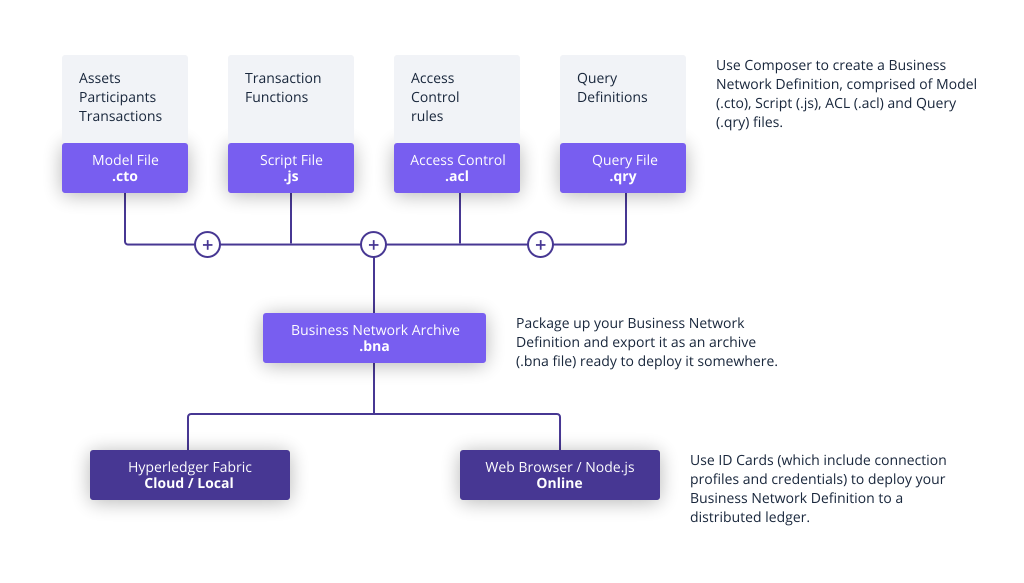
\includegraphics[width=\textwidth]{graphics/Composer-Diagram.png}
    		\caption[Bestandteile einer Hyperledger Composer-Applikation]{Bestandteile einer Hyperledger Composer-Applikation\cite{ComposerDocs}}
    		\label{fig:composer_arch}
    	\end{figure}
        
        \begin{itemize}[noitemsep]
            \item Möglichkeit eine REST-\gls{api} pro Business Network Card mit folgenden Features zu generieren
                \begin{itemize}[noitemsep]
                    \item Nutzung von API-Keys für die Sicherung der REST-\gls{api}
                    \item Authentifizierung via Passport auf Linux-Maschinen
                    \item ,,Explorer Test Interface``, welches automatisch generiert wird und essentiell eine Dokumentation der \gls{api} darstellt mit der zusätzlichen Möglichkeit die \gls{api}-Calls zu testen.
                    \item Key für dynamisches Logging
                    \item Event Publication via WebSocket
                    \item \gls{tls} und HTTPS für die \gls{api}
                \end{itemize}
            \item Bietet die Möglichkeit eine simple Anuglar-App zu generieren, welche letztendlich nur eine GUI-Maske für die \gls{api}-Methoden ist.
            \item Actors im Netzwerk (Peers, Orderers, Client Applications etc. haben eine digitale Identität, welche sich in einem X.509 digitalem Zeritifikat befindet.
                Die Zertifikate sind letztendlich ausschlaggebend für die Zugriffskontrolle und den Rechten, die eine Entität in dem Netzwerk erhält. 
                Zusätzlich können weitere Attribute, die zu einer Identät gehören genutzt werden (wie bspw. Organisiation, Rolle, etc.), welche eine Rolle bei der Bestimmung, welche Rechte diese Entität erhalten soll, spielen können.
            \item Zertifikate kommen von einer vertrausenswürdigen Autortität, dem \gls{msp}. 
                Gleicht einer PKI mit digitalen Zertifikaten, public/\-private Keys, CA und CRL
            \item öffentliche und private Kanäle: Nachrichtenwege, um Privatsphäre von Transaktionen und Vertraulichkeit zu gewährleisten.
                Private Kanäle sind nur für bestimmte Netzwerkmitglieder sichtbar, denen der Channel freigegeben wurde.
            \item Ordering Service: ein oder mehrere Knoten, die Transaktionen in einem Block ordnen
            \item Ledger: Blockchain + World State
            \item Deployable: Business Network Archive (bna)
            \item Historian: registry which records successful transactions, including the participants and identities that submitted them
        \end{itemize}
        
        \begin{itemize}[noitemsep]
            \item Single Organization 
            \item Membership Provider Service
        \end{itemize}
    

    \subsection{Architektur, Funktionsweise und Implementierung}
\label{sec:prototype_arch} 
    Da momentan weder eine Standardisierung noch Best Practices von Blockchainarchitekturen existieren, wurde die Architektur des Prototypen anhand der Dokumentation des Frameworks\cite{ComposerDocs}, sowie den darin enthaltenen Beispielen ausgearbeitet. 
    Sollte eine Beschreibung direkt auf einen der beiden Anfoderungskataloge, die in \fref{sec:prototype_func_req} und in \fref{sec:prototype_sec} gesammelt wurden beziehen, so wird diese mit der entsprechenden Referenz verdeutlicht.
    
    \subsubsection{Konzept}
        Das Blockchain-Netzwerk für den Prototypen umfasst ein oder mehrere Herstellerserver, ein oder mehrere Schlösser, sowie ein oder mehrere Nutzer und basiert auf einer private/permissioined Blockchain. 
        Sollten Alice und Bob je ein Schloss vom gleichen Hersteller haben, aber nicht im gleichen ,,Haus`` wohnen, so entstehen zwei unterschiedliche Blockchain-Netzwerke, die jeweils voneinander isoliert sind.
        \smallskip\\
        \noindent Im Modell des Prototypen gibt es demnach drei verschiedene Teilnehmertypen, wobei für ein minimales funktionales Netzwerk mindestens Teilnehmer jedes Typs vertreten sein muss. 
        In dem Netzwerk kann jeder Teilnehmer mit allen anderen Teilnehmern kommunizieren.
        \begin{enumerate}[noitemsep]
            \item \textbf{Hersteller/Vendor}: Zur Initialisierung, Zurücksetzung, Updates, \dots
            \item \textbf{Schloss/Lock}: das physische Schloss, welches bei einem Nutzer installiert wird
            \item \textbf{Nutzer/User}: öffnet/schließt ein oder mehrere Schlösser, verwaltet u.U. andere Nutzer
        \end{enumerate}
        
        \noindent In \fref{fig:pt_network} ist ein Beispiel mit zwei verschiedenen Herstellern \colorbox{light-gray}{\lstinline{V1,V2}}, drei Schlössern \colorbox{light-gray}{\lstinline{L1,L2,L3}} und drei Nutzern \colorbox{light-gray}{\lstinline{U1,U2}}. 
        Insgesamt wurden vier Schlüssel \colorbox{light-gray}{\lstinline{K1-K4}} ausgestellt.
        \colorbox{light-gray}{\lstinline{L1}} und \colorbox{light-gray}{\lstinline{L2}} sind von Hersteller \colorbox{light-gray}{\lstinline{V1}}, \colorbox{light-gray}{\lstinline{L3}} stammt von Hersteller \colorbox{light-gray}{\lstinline{H2}}. 
        \colorbox{light-gray}{\lstinline{U1}} hat mit den beiden Schlüsseln \colorbox{light-gray}{\lstinline{K1,K2}} die Möglichkeit \colorbox{light-gray}{\lstinline{L1}} und \colorbox{light-gray}{\lstinline{L3}} zu öffnen. 
        Der Nutzer \colorbox{light-gray}{\lstinline{U2}} kann mit \colorbox{light-gray}{\lstinline{K3}} und \colorbox{light-gray}{\lstinline{K4}} die Schlösser \colorbox{light-gray}{\lstinline{L2}} und \colorbox{light-gray}{\lstinline{L3}} öffnen.
        \begin{figure}[H]
    		\centering
    		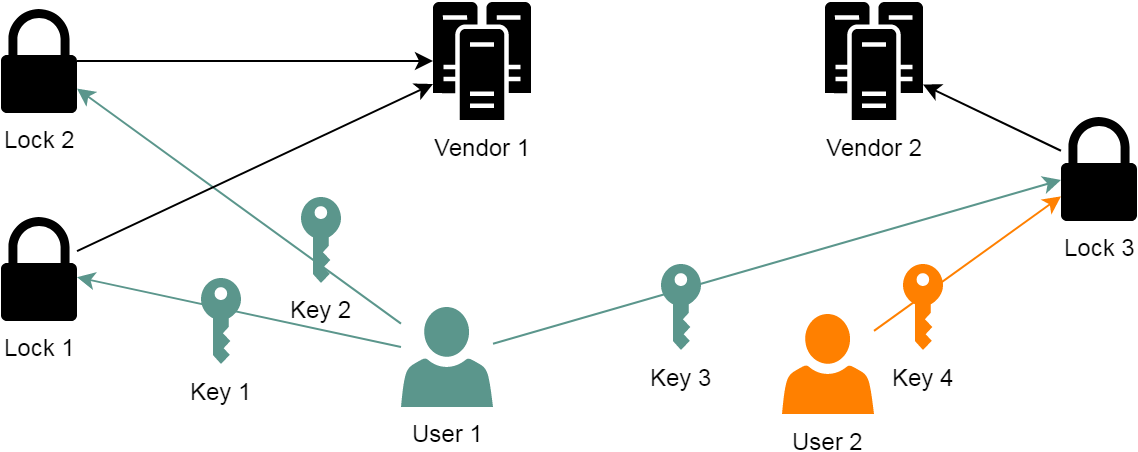
\includegraphics[width=\textwidth]{graphics/pt_network.png}
    		\caption[Beispiel eines von Beziehungen im Prototypen-Netzwerk]{Beispiel von Beziehungen eines Netzwerks, welches aus der Definition des Prototypen entstehen könnte}
    		\label{fig:pt_network}
    	\end{figure}
        \noindent Je nach Teilnehmertyp werden erlaubte Operationen innehalb des Netzwerkes mittels der \gls{acl} eingeschränkt. 
        Die Zugriffskontrolle für den Teilnehmertyp ,,Nutzer`` erfolgt zusätzlich auf einer feingranulareren Ebene über ein dafür angelegtes Attribut \colorbox{light-gray}{\lstinline{UserRole}} mit dem in \fref{tab:prototype_rbac} dargestellten Berechtigungskonzept. 
        Es ist rollenbasiert und ist wurde analog zu \fref{tab:rbac} entworfen. 
        Anders ist jedoch, dass angelehnt an öffentliche Netzwerke, alle Nutzer des Netzwerkes alle Informationen, die in dieser gespeichert wurden einsehen, aber nicht verändern können. 
        Wie in \fref{tab:prototype_rbac} verdeutlicht, gibt es die Rollen ,,Besitzer`` und ,,Gast`` mit unterschiedlichen Berechtigungen (\ref{fa:3}, \ref{fa:4}). 
        \begin{table}[H]
		    {\footnotesize
		    \centering
            \begin{tabular}{|m{0.14\textwidth}|m{0.14\textwidth}|m{0.14\textwidth}|m{0.14\textwidth}|m{0.14\textwidth}|m{0.14\textwidth}|}
                \hline
                \textbf{Rolle/Recht} &\textbf{Unlock}  & \textbf{Log einsehen}  & \textbf{Nutzer verwalten}  & \textbf{Rollen\-verwal\-tung} & \textbf{Schloss zurück\-setzen}  \\ \hline
                \textbf{Owner}       & \checkmark      & \checkmark             & \checkmark                 & \checkmark                    & \checkmark                       \\ \hline
                \textbf{Guest}       & \checkmark      & \checkmark             & ~                          & ~                             & ~                                \\ \hline
            \end{tabular}
            }
            \caption[Rollenbasierte Zugangskontrolle des Prototypen]{Rollenbasierte Zugangskontrolle des Prototypen. Ist ein Haken gesetzt, so wird der Rolle in der Spalte links das Recht aus der entsprechnenden Spalte gewährt.}
            \label{tab:prototype_rbac}
        \end{table}
        \noindent Schlüssel werden als Asset repräsentiert und von Nutzern verwendet, um ein Schloss zu öffnen(\ref{fa:2}). 
        Optional können die Schlüssel mit einem Ablaufzeitpunkt zeitlich eingeschränkt sein(\ref{fa:5}). 
        Es wird ein Schlüssel je Nutzer und Schloss ausgestellt. 
        Somit gäbe es beispielsweise bei zwei Schlössern \colorbox{light-gray}{\lstinline{L1,L2}} und einem Nutzer \colorbox{light-gray}{\lstinline{U1}} im Netzwerk zwei Schlüssel: \colorbox{light-gray}{\lstinline{U1arwL1,U1arwL2}}. \\
        Schlüssel sind nach Erstellung nicht modifizierbar und werden, falls ein Ablaufzeitpunkt angegeben wurde gelöscht. 
        Beim Öffnen des Schlosses geprüft, ob der öffende Nutzer das entsprechende Schlüsselasset besitzt und im Schloss eine Referenz auf den Schloss gespeichert. 
        Wird das Schloss wieder verriegelt, so wird die Referenz wieder gelöscht. 
        Hiermit kann einerseits sichergestellt werden, dass das Schloss geschlossen ist, wenn dieses keine Referenzen auf Schlüsselassets besitzt, andererseits wird jegliche Nutzung des Schlosses auf der Blockchain dokumentiert. 
        \medskip\\
        \noindent Mittels der in \fref{sec:prototype_composer} vorgestellten Mechanik des Historians werden nach diesem Konzept folgende Informationen also in der Blockchain gespeichert:
        \begin{itemize}[noitemsep]
            \item Erstellen, Modifizieren und Löschen von Ressourcen (Vendor, Lock, User, Key)
            \item Wann von wem welches Schloss geöffnet wurde und welchen Zustand dieses hat
            \item Welche Person welche Rolle inne hat und von wem diese gewährt wurde
            \item Jegliche erfolgreich abgeschlossenen Transaktionen
        \end{itemize}
        
    \subsubsection{Implementierungs- und Konfigurationsdetails}
        Die drei Teilnehmertypen werden jeweils als \colorbox{light-gray}{\lstinline{participant}}-Ressourcen modelliert und können somit von Entitäten, die an dem Netzwerk teilnehmen wollen (beispielsweise eine Person mit Smartphone-App, ein Smart Lock-Gerät oder ein Server des Herstellers), dafür genutzt werden. 
        \medskip\\
        Im Framework werden alle Ressourcen auch über eine \colorbox{light-gray}{\lstinline{ID}} identifiziert, welche bei der Erstellung dieser selbst gewählt werden muss. 
        Generierte \colorbox{light-gray}{\lstinline{IDs}} sind insofern sicherheitsrelevant, dass sie, durch beispielsweise automatisch hochzählende Werte, anfällig für eine Enumerationschwachstelle sind. 
        Für diesen Prototypen werden jegliche \colorbox{light-gray}{\lstinline{IDs}} mittels der Crypto-\gls{api}, welche von der JavaSript-Laufzeitumgebung bereitgestellt wird, erstellt.
        \medskip
        \begin{lstlisting}[caption={Repräsantation eines Nutzers},label=prototype_user,captionpos=b]
participant User identified by userId {
    o String userId
    o String firstName
    o String lastName
    o String email
    o UserRole role
    --> LockKey[] keys optional
}
        \end{lstlisting}
        
        \noindent Weitere Attribute einer Repräsentation eines Nutzers in Listing \ref{prototype_user} sind Vor- und Nachname, E-Mailadresse und, falls vorhanden, ein Array mit Referenzen auf Schlüssel, die der Nutzer besitzt. 
        Die Rolle des Nutzers kann dem Berechtigungskonzept nach lediglich die Werte \colorbox{light-gray}{\lstinline{GUEST}} und \colorbox{light-gray}{\lstinline{OWNER}} annehmen. 
        \medskip
        \begin{lstlisting}[caption={Repräsantation eines Herstellers},label=prototype_vendor,captionpos=b]
participant Vendor identified by vendorId {
    o String vendorId
    --> Lock[] locks
}
        \end{lstlisting}
        Ein Hersteller (vgl. Listing \ref{prototype_vendor}) hat im Prototypen zusätzlich zur zugewiesenen \colorbox{light-gray}{\lstinline{ID}} eine Liste registierter Schlösser.
        \medskip
        \begin{lstlisting}[caption={Repräsantation eines Schlosses},label=prototype_lock,captionpos=b]
participant Lock identified by lockId {
    o String lockId
    o String name
    o LockState state
    --> LockKey[] keyInUse
    --> Vendor vendor
}
        \end{lstlisting}
        Um die Benutzerfreundlichkeit zu gewährleisten hat jedes Schloss einen beliebig wählbaren Namen zusätzlich zur \colorbox{light-gray}{\lstinline{ID}}, dessen Zustand (\colorbox{light-gray}{\lstinline{UNLOCKED}},\colorbox{light-gray}{\lstinline{LOCKED}}) und der Referenz auf den Hersteller. 
        Ein Array, welches, sofern das Schloss geöffnet ist, eine Referenz auf den zum Öffnen verwendeten Schlüssel enthält, wird stets so validiert, dass es lediglich 0 oder 1 Elemente enthält.
        
        %%%%%%%%%%%%%%%%%%%%%%%%%%%%%%%%%%%%%%%%%%%%%%%%%%%%%%%%%%%%%%%%%%%%
            
            Asset Types:
            \begin{lstlisting}[caption={Asset Types},label=prototype_assets,captionpos=b]
asset LockKey identified by keyId {
    o String keyId
    o DateTime expirationDate optional
    --> Lock lock
    --> User owner
    --> User issuer
}
            \end{lstlisting}
        
            Transaction Types:
            \begin{lstlisting}[caption={Relevante Transaktionen},label=prototype_transactions,captionpos=b]
transaction ResetLock {
    --> Lock lock
}

transaction RemoveLock {
    --> Lock lock
}

transaction RegisterLock {
    --> Lock lock
}

transaction InitializeNetwork {
    o String firstName
    o String lastName
}

transaction Unlock {
    --> Lock lock
}

transaction CloseLock {
    --> Lock lock
}

transaction GrantUnlock {
    --> Lock lock
    o DateTime expirationDate optional
    --> User grantee
}

transaction RevokeUnlock {
    --> Lock lock
    --> User revokee
}

transaction GrantOwner {
    --> User grantee
}

transaction RevokeOwner {
    --> User revokee
}


            \end{lstlisting}
            
            \begin{itemize}[noitemsep]
                \item Transaktionen bekommen aus dem Systemnamespace schon einen Timestamp und eine ID
                \item OpenDoor
                \item User (AddUser, DeleteUser, ChangeUserRole)
                \item TimeSlot (AddTimeSlot, DeleteTimeSlot, ChangeGuestTimeSlot)
            \end{itemize}
    
    \paragraph{\textrm{Transaction Functions}}
    
    \paragraph{\textrm{Access Control Rules}}\hspace{0cm}\\
        Die Vorgehensweise bei der Definition der \gls{acl}s ist sogenanntes ,,Whitelisting``. 
        Es werden also grundsätzlich alle Operationen auf alle Ressourcen verboten und nur einzelne bestimmte Aktionen von bestimmten Teilnehmern, teilweise nur unter bestimmten Bedinungen erlaubt. 
        Da in Hyperledger Composer die einzelnen Regeln geordnet nacheinander evaluiert werden, müssen zunächst alle erlaubten Aktionen definiert und zum Schluss alle verweigert werden. 
        Eine ausführliche auflistung aller Regeln befindet sich im Anhang\todo[color=orange]{Referenz einfügen}. 
        Beispielsweise:
        \missingfigure{Komplettes Regelwerk für eine Ressource als Beispiel}
        \begin{lstlisting}[caption={Relevante Transaktionen},label=prototype_acl,captionpos=b]
// Asset: LockKey
rule OwnerCanIssueLockKey {
    description: "owners can issue lock keys to users"
    participant(u): "de.hftl.user.User"
    operation: CREATE
    resource(k): "de.hftl.lock.LockKey"
    transaction(tx): "de.hftl.permissions.GrantUnlock"
    condition: (
        u.role == "OWNER"
    )
    action: ALLOW
}

rule OwnerCanDeleteLockKey {
    description: "owners can delete lock keys"
    participant(u): "de.hftl.user.User"
    operation: DELETE
    resource(k): "de.hftl.lock.LockKey"
    transaction(tx): "de.hftl.permissions.RevokeUnlock"
    condition: (
        u.role == "OWNER"
    )
    action: ALLOW
}

rule AnyoneCanSeeTheKeys {
    description: "any participant can see all keys"
    participant: "de.hftl.**"
    operation: READ
    resource: "de.hftl.lock.LockKey"
    action: ALLOW
}

rule DenyKeyModifications {
    description: "no one can modify or delete keys"
    participant: "de.hftl.**"
    operation: CREATE,UPDATE, DELETE
    resource: "de.hftl.lock.LockKey"
    action: DENY
}
        \end{lstlisting}
        
    \paragraph{Query Definitions}
    

    Notizen für den Prototypen:
    \begin{itemize}[noitemsep]
        \item How to ensure a consistent state across all entities?...
        \item keine Anonymisierung, da der Access Log auditable sein muss
        \item Hyperledger bietet CA für Identitäten, Authentifizierung \textrightarrow\ wie ist das bei Composer?
        \item \begin{itemize}
            \item erlaubt Sicherheitseinstellungen beim Erstellen des REST-API-Servers
            \item API Key
            \item Authentication mit Passport
            \item explorer Test interface ?
            \item dynamic logging
            \item event publication over websockets
            \item TLS enable/\-disable
        \end{itemize}
    \end{itemize}
    
    \newpage
    \section{Evaluation des Prototypen}
\label{sec:evaluation}
    \newpage
    \section{Vergleich des Prototypen mit den Analyseergebnissen}
\label{sec:comparison}
Vergleich beider Ergebnisse anhand der Kategorien.

    \newpage
    \section{Ergebnis}
\label{sec:end}
    Allgemein lässt sich daraus erkennen, dass die meisten Schwachstellen, bis auf eine Ausnahme, die im Prototypen existieren mittels \gls{cvss} ,,Low`` und ,,Medium`` bewertet werden.
    \medskip\\
    Vergleich anhand er Kategorien
    \bigskip\\
    Die Probleme der Proxy-Architektur wären damit beseitigt, aber jedoch bleiben die Probleme der direkten Architektur erhalten.

%%%%%%%%%%%%%%%%%%%%%%%%%%%%%%%%%%%%%%%%
\hspace{0cm}\bigskip\\
    Abwägungen zum Einsatz der Blockchain-Technologie im \gls{iot}
    \begin{itemize}[noitemsep]
        \item Blockchain tut sehr viel in Richtung Identity Management, nützt aber nichts, wenn das Umfeld (Übertragung via HTTP und nicht HTTPS, keine 2-Factor Authentication, etc.) nicht gesichert ist.
        \item kurz Vorteile/Nachteile von Blockchain
        \item Manche Anforderungen aus \fref{sec:prototype_requirements} nicht direkt umsetzbar.
            Einige dieser sind dennoch essentiell für die Sicherheit einer \gls{iot}-Applikation.
        \item Grenzen der Aussagekraft des Prototypen
		    \begin{itemize}[noitemsep]
		        \item Mindestanzahl an Teilnehmern im Blockchain-Netzwerk wegen \gls{bft} \textrightarrow andere Konsensalgorithmen bzw. -mechanismen
		        \item Privatsphäre in private Blockchains
		        \item Passwortrücksetzung
		        \item falsche Sicherheitskonfigurationen auf Host des Prototypen kann nicht betrachtet werden
		    \end{itemize}
		\item Worüber keine Aussagen getroffen werden konnten, z.B. Automatisches Öffnen-/\-Schließen konnte gar nicht getestet werden
    \end{itemize}
    Daher lohnt es sich nach der Untersuchung (oder lohnt es sich nicht) innerhalb des Rahmens dieser Arbeit die Blockchain-Technologie im \gls{iot}, spezifisch bei Smart Locks einzusetzen.
    
    
\section{Ausblick}
\label{sec:end_further}
	\begin{itemize}[noitemsep]
		\item Auf die Konzepte Self-Sovereign Identitiy, Decentralized Identifiers eingehen und referenzieren
		\item Ideen zur sicherheitstechnischen Erweiterung des Prototypen erläutern
		\begin{itemize}[noitemsep]
		    \item Event, wenn der Schlüssel häufiger als X mal pro Stunde oder Tag benutzt werden
		    \item Granularere Verteilung der Rollen im Netzwerk, auf einzelne Locks jeweils Owner und Guest Rollen
		    \item Security events generieren, welche von den jeweiligen Ownern eingesehen werden können und somit alarmier werden
		    \item Inputvalidierungen bei Nutzereingaben
		    \item Skalierung? Wenn der Hersteller für viele Kunden jeweils einen eigenen Knoten betreiben muss
		\end{itemize}
	\end{itemize}

    %\nocite{*}

	%!!!!!!!!!!!!!!!!!!!!!!!!BIS HIER ARBEITEN!!!!!!!!!!!!!!!!!!!!!!!!
	%########################################################################################################
    \newpage	
    \printbibliography[title=Literaturverzeichnis]

    %% ANHANG 
    \newpage
    \appendix
    \renewcommand{\thesection}{\Roman{section}}
    \appendixpage
    \addappheadtotoc
    \section{Details CVSS}
    Put this shit here.\todo[color=cyan]{Details einfügen}
\newpage
\section{CVSS-Score Tabellen}
    Die verwendeten Abkürzungen aus den in \fref{sec:sota_sa_cvss} vorgestellen Variablen:
    \begin{itemize}[noitemsep]
        \item Attack Vector(AV): Network(N), Adjacent(A), Local(L), Physical(P)
        \item Attack Complexity(AC)
        \item Privileges Required(PR)
        \item User Interaction
        \item usw. \todo[color=orange]{ausfüllen}
    \end{itemize}

\begin{sidewaystable}
\centering
\begin{tabularx}{\textwidth}{|l|X|X|X|X|X|X|X|X|l|}
\hline
                                                     & \textbf{AV} & \textbf{AC} & \textbf{PR} & \textbf{UI} & \textbf{S} & \textbf{C} & \textbf{I} & \textbf{A} & \textbf{Score} \\ \hline
\textbf{{[}I1{]} Insecure API}                       & P           & L           & N           & N           & C          & N          & H          & N          & 5.3            \\ \hline
\textbf{{[}I2{]} Insufficient Password Prototection} & N           & H           & N           & R           & C          & L          & H          & N          & 6.9            \\ \hline
\textbf{{[}I2{]} API: Privilege Escalation}          & N           & L           & N           & N           & C          & L          & H          & N          & 9.3            \\ \hline
\textbf{{[}I2{]} Insecure Password Policy}           & N           & H           & N           & N           & U          & L          & L          & N          & 4.8            \\ \hline
\textbf{{[}I2{]} Phishing}                           & L           & H           & N           & R           & C          & N          & H          & N          & 5.5            \\ \hline
\textbf{{[}I2{]} Replay}                             & L           & H           & N           & R           & C          & H          & N          & N          & 5.5            \\ \hline
\textbf{{[}I2{]} Device Spoofing}                    & N           & H           & N           & N           & U          & H          & L          & L          & 7.0            \\ \hline
\textbf{{[}I2{]} Missing 2-Factor Authentication}    & P           & H           & L           & N           & C          & H          & H          & N          & 6.7            \\ \hline
\textbf{{[}I3{]} DoS via Commands}                   & A           & H           & H           & N           & U          & N          & N          & H          & 4.2            \\ \hline
\textbf{{[}I3{]} DoS via Manufacturer}               & N           & H           & N           & N           & U          & N          & N          & H          & 5.9            \\ \hline
\textbf{{[}I3{]} DoS via Blueooth}                   & A           & L           & N           & N           & U          & N          & N          & H          & 6.5            \\ \hline
\textbf{{[}I3{]} Access Log Evasion}                 & A           & L           & L           & N           & U          & N          & H          & N          & 5.7            \\ \hline
\textbf{{[}I4{]} Insecure Password Transmission}     & A           & L           & N           & R           & U          & N          & L          & N          & 3.5            \\ \hline
\textbf{{[}I4{]} Revocation Evasion}                 & A           & L           & L           & N           & U          & N          & H          & N          & 6.5            \\ \hline
\textbf{{[}I4{]} Decompiling APKs}                   & A           & H           & N           & R           & U          & H          & H          & N          & 6.4            \\ \hline
\textbf{{[}I5{]} Extracted User Data}                & L           & H           & H           & N           & U          & H          & H          & L          & 6.0            \\ \hline
\textbf{{[}I7{]} Stolen User Settings}               & L           & H           & H           & N           & U          & H          & H          & L          & 6.0            \\ \hline
\textbf{{[}I7{]} Insecure Bluetooth Pairing}         & A           & H           & N           & R           & C          & H          & H          & L          & 7.8            \\ \hline
\textbf{{[}I9{]} Fuzzing}                            & A           & H           & N           & R           & U          & H          & H          & H          & 7.1            \\ \hline
\end{tabularx}
\caption{Detaillierte Ergebnisse der Bewertung in \fref{sec:analysis_cvss}}
\label{tab:analysis_cvss_long}
\end{sidewaystable}
\newpage


\begin{sidewaystable}
\centering
\begin{tabularx}{\textwidth}{|l|X|X|X|X|X|X|X|X|l|}
\hline
\textbf{}                                      & \textbf{AV} & \textbf{AC} & \textbf{PR} & \textbf{UI} & \textbf{S} & \textbf{C} & \textbf{I} & \textbf{A} & \textbf{Score} \\ \hline
\textbf{{[}I2{]} ID-Card Theft}                & A           & H           & N           & N           & C          & H          & H          & L          & 8.2            \\ \hline
\textbf{{[}I2{]} Single Point of Failure}      & L           & H           & L           & N           & U          & L          & H          & L          & 5.8            \\ \hline
\textbf{{[}I3{]} DoS via REST-Server}          & L           & H           & N           & N           & U          & N          & N          & L          & 2.9            \\ \hline
\textbf{{[}I5{]} Unprotected User Information} & L           & H           & L           & N           & U          & H          & N          & N          & 4.7            \\ \hline
\textbf{{[}I6{]} Participant Enumeration}      & L           & L           & L           & N           & U          & L          & N          & N          & 3.3            \\ \hline
\textbf{{[}I6{]} Asset Enumeration}            & L           & L           & L           & N           & U          & L          & N          & N          & 3.3            \\ \hline
\textbf{{[}I8{]} Unencrypted Data Storage}     & L           & L           & L           & N           & U          & H          & N          & N          & 5.5            \\ \hline
\textbf{{[}I9{]} Insufficient Sandboxing}      & L           & L           & H           & N           & U          & L          & L          & L          & 4.2            \\ \hline
\textbf{{[}I9{]} Log Injection}                & L           & L           & L           & N           & U          & N          & L          & N          & 3.3            \\ \hline
\textbf{{[}I9{]} Code Injection}               & L           & L           & L           & N           & U          & N          & L          & N          & 3.3            \\ \hline
\end{tabularx}
\caption{Detaillierte Ergebnisse der Bewertung in \fref{sec:evaluation_cvss}}
\label{tab:eval_cvss_long}
\end{sidewaystable}


\newpage

    %\section{Source Code des Prototypen}
    Der Source Code des Prototypen ist unter \sloppy\url{https://github.com/qn0x/smart-lock-prototype} zu finden. 
    Zudem sind im Folgedenden die wichtigsten Bestandteile des Prototypen angehängt.
    
    \subsection{Modelle}
        \begin{lstlisting}[caption={Assets},label=model_assets,captionpos=b]
asset LockKey identified by keyId {
    o String keyId
    o DateTime expirationDate
    o DateTime lastUsed
    --> Lock lockId
    --> User owner
    --> User issuer
}
        \end{lstlisting}
        \vspace{1em}
        \begin{lstlisting}[caption={Participants},label=model_participants,captionpos=b]
participant User identified by userId {
    o String userId
    o String firstName
    o String lastName
    o UserRole role
}

participant Lock identified by lockId {
    o String lockId
    o String name
    o DateTime lastUnlocked
    o LockState state
}

enum UserRole {
  o USER
  o ADMIN
}

enum LockState {
  o UNLOCKED
  o LOCKED
}
        \end{lstlisting}
        \vspace{1em}
        \begin{lstlisting}[caption={Transactions},label=model_transactopms,captionpos=b]
transaction Unlock {
    --> LockKey lockKey
    --> Lock lock
}

transaction GrantUnlock {
    --> LockKey lockKey
    --> Lock lock
    --> User issuer
    --> User grantee
}

transaction RevokeUnlock {
    --> LockKey lockKey
    --> Lock lock
    --> User issuer
    --> User revokee
}

transaction GrantAdmin {
    --> User issuer
    --> User grantee
}

transaction RevokeAdmin {
    --> User issuer
    --> User revokee
}
        \end{lstlisting}
    
    \subsection{Access Control}
    \subsection{Transaktionslogik}
\newpage
\section{Verwendung des Prototypen}
    For Dummies. 


\end{document}
